\PassOptionsToPackage{unicode=true}{hyperref} % options for packages loaded elsewhere
\PassOptionsToPackage{hyphens}{url}
%
\documentclass[]{book}
\usepackage{lmodern}
\usepackage{amssymb,amsmath}
\usepackage{ifxetex,ifluatex}
\usepackage{fixltx2e} % provides \textsubscript
\ifnum 0\ifxetex 1\fi\ifluatex 1\fi=0 % if pdftex
  \usepackage[T1]{fontenc}
  \usepackage[utf8]{inputenc}
  \usepackage{textcomp} % provides euro and other symbols
\else % if luatex or xelatex
  \usepackage{unicode-math}
  \defaultfontfeatures{Ligatures=TeX,Scale=MatchLowercase}
\fi
% use upquote if available, for straight quotes in verbatim environments
\IfFileExists{upquote.sty}{\usepackage{upquote}}{}
% use microtype if available
\IfFileExists{microtype.sty}{%
\usepackage[]{microtype}
\UseMicrotypeSet[protrusion]{basicmath} % disable protrusion for tt fonts
}{}
\IfFileExists{parskip.sty}{%
\usepackage{parskip}
}{% else
\setlength{\parindent}{0pt}
\setlength{\parskip}{6pt plus 2pt minus 1pt}
}
\usepackage{hyperref}
\hypersetup{
            pdftitle={Brain and Body Lab},
            pdfborder={0 0 0},
            breaklinks=true}
\urlstyle{same}  % don't use monospace font for urls
\usepackage{longtable,booktabs}
% Fix footnotes in tables (requires footnote package)
\IfFileExists{footnote.sty}{\usepackage{footnote}\makesavenoteenv{longtable}}{}
\usepackage{graphicx,grffile}
\makeatletter
\def\maxwidth{\ifdim\Gin@nat@width>\linewidth\linewidth\else\Gin@nat@width\fi}
\def\maxheight{\ifdim\Gin@nat@height>\textheight\textheight\else\Gin@nat@height\fi}
\makeatother
% Scale images if necessary, so that they will not overflow the page
% margins by default, and it is still possible to overwrite the defaults
% using explicit options in \includegraphics[width, height, ...]{}
\setkeys{Gin}{width=\maxwidth,height=\maxheight,keepaspectratio}
\setlength{\emergencystretch}{3em}  % prevent overfull lines
\providecommand{\tightlist}{%
  \setlength{\itemsep}{0pt}\setlength{\parskip}{0pt}}
\setcounter{secnumdepth}{5}
% Redefines (sub)paragraphs to behave more like sections
\ifx\paragraph\undefined\else
\let\oldparagraph\paragraph
\renewcommand{\paragraph}[1]{\oldparagraph{#1}\mbox{}}
\fi
\ifx\subparagraph\undefined\else
\let\oldsubparagraph\subparagraph
\renewcommand{\subparagraph}[1]{\oldsubparagraph{#1}\mbox{}}
\fi

% set default figure placement to htbp
\makeatletter
\def\fps@figure{htbp}
\makeatother

\usepackage{booktabs}
\usepackage{amsthm}
\makeatletter
\def\thm@space@setup{%
  \thm@preskip=8pt plus 2pt minus 4pt
  \thm@postskip=\thm@preskip
}
\makeatother
\usepackage[]{natbib}
\bibliographystyle{apalike}

\title{Brain and Body Lab}
\author{}
\date{\vspace{-2.5em}}

\begin{document}
\maketitle

{
\setcounter{tocdepth}{1}
\tableofcontents
}
\hypertarget{introduction}{%
\chapter{Introduction}\label{introduction}}

\begin{center}\rule{0.5\linewidth}{0.5pt}\end{center}

Welcome to the BABLab Wiki!

In the Brain and Body Lab we are interested in how early experiences influence interactions between the brain and body, contributing to mental and physical health. We hope to use this information to improve the wellbeing of children, adolescents, and adults across the world. In other words, in the BABLab, we aim to do good science that makes a difference to people's lives, today and tomorrow.

The BABLab is directed by Dr.~Bridget Callaghan, Assistant Professor of Psychology at UCLA.

\textbf{Current Projects:}

\begin{itemize}
\tightlist
\item
  \href{https://bab-lab.github.io/mind_brain_body/}{Mind, Brain, Body (MBB)}
\item
  \href{https://osf.io/nf2bv/}{EGG and Emotionality (EGG)}
\item
  Transfer Mental Health
\end{itemize}

\hypertarget{finding-the-lab}{%
\section{Finding the Lab}\label{finding-the-lab}}

We're located in the Psychology Department at UCLA!
5581 Pritzker Hall
This is in the tower building, 5th floor.

\hypertarget{contact-info}{%
\section{Contact Info}\label{contact-info}}

If you have any questions about the lab please contact the lab's managers.

Emily Towner - \href{mailto:emilytowner@ucla.edu}{\nolinkurl{emilytowner@ucla.edu}}.
Kristen Chu - \href{mailto:kristenchu@g.ucla.edu}{\nolinkurl{kristenchu@g.ucla.edu}}

Alternatively, you can reach out to our lab email, \href{mailto:bablab.ucla@gmail.com}{\nolinkurl{bablab.ucla@gmail.com}}

\hypertarget{other-information}{%
\section{Other Information}\label{other-information}}

Feel free to contribute any relevant sections or information - best lunch spots on campus, tips and tricks, or anything else helpful to your fellow lab members!

\hypertarget{onboarding}{%
\chapter{Onboarding}\label{onboarding}}

\begin{center}\rule{0.5\linewidth}{0.5pt}\end{center}

\hypertarget{first-steps}{%
\section{First Steps}\label{first-steps}}

If you are a new member of the BAB Lab, there are a few basic things you will want to set up before or on your first day.

\textbf{Here are some tips:}

\begin{enumerate}
\def\labelenumi{\arabic{enumi}.}
\item
  Read the \href{https://bab-lab.github.io/lab_manual/}{Lab Manual}
\item
  Ask the lab manager to be added to the following
\end{enumerate}

\begin{itemize}
\tightlist
\item
  \href{https://slack.com/}{Slack} (download the desktop and mobile \href{https://slack.com/downloads/mac}{apps})
\item
  \href{https://trello.com/emilyanntowner/boards}{Trello} (download the desktop and mobile \href{https://trello.com/en-US/platforms}{apps} - watch this \href{https://www.youtube.com/watch?v=_Ry-SnJygy8\&feature=youtu.be}{tutorial})
\item
  Box
\item
  Google calendars
\item
  Email list
\item
  Dropbox Paper
\end{itemize}

\begin{enumerate}
\def\labelenumi{\arabic{enumi}.}
\setcounter{enumi}{2}
\tightlist
\item
  Send (via Slack) the lab manager your information including your
\end{enumerate}

\begin{itemize}
\tightlist
\item
  Preferred name
\item
  Preferred email
\item
  Phone number
\item
  Photo
\item
  Brief bio for the lab website
\end{itemize}

\begin{enumerate}
\def\labelenumi{\arabic{enumi}.}
\setcounter{enumi}{3}
\tightlist
\item
  Complete the onboarding process for your position below
\end{enumerate}

\begin{center}\rule{0.5\linewidth}{0.5pt}\end{center}

\hypertarget{onboarding---staff-research-associate}{%
\section{Onboarding - Staff Research Associate}\label{onboarding---staff-research-associate}}

\begin{enumerate}
\def\labelenumi{\arabic{enumi}.}
\tightlist
\item
  Submit to Bridget

  \begin{itemize}
  \tightlist
  \item
    Signed employment contract
  \end{itemize}
\item
  Contact HR

  \begin{itemize}
  \tightlist
  \item
    Human Resources Coordinator
  \item
    1283A Franz Hall
  \item
    (310) 206-9720
  \end{itemize}
\item
  Submit to HR

  \begin{itemize}
  \tightlist
  \item
    \href{https://ucla.app.box.com/s/z58tkq6l13qwl0zw5gtqhdxq0cne1wcu}{Union overtime/comp form}
  \item
    \href{https://ucla.app.box.com/s/7jmouwl8fbp5039qq4tfmreo5r5ydmjq}{Personal data form}
  \item
    \href{https://ucla.app.box.com/s/tothrcm0zcz50hj829bkcj1idclcudzr}{Background check authorization form}
  \end{itemize}
\item
  Schedule with HR

  \begin{itemize}
  \tightlist
  \item
    Background check phone call
  \item
    Hiring meeting
  \item
    Bring employment verification \href{https://ucla.app.box.com/s/iwguajwkedo2zf2lfr5ie3z5tc4vnz7m}{documents} to meeting (i.e.~passport)
  \item
    Sign \href{https://ucnet.universityofcalifornia.edu/forms/pdf/upay-585.pdf}{state oath of allegiance/patent policy/patent acknowledgment} (in person)
  \end{itemize}
\item
  Pick-up

  \begin{itemize}
  \tightlist
  \item
    Location: Psychology Main Office (1285 Psychology Building -- See Tyler Tuione)

    \begin{itemize}
    \tightlist
    \item
      Parking permits
    \end{itemize}
  \end{itemize}
\item
  Respond

  \begin{itemize}
  \tightlist
  \item
    To the tracker I-9 email on or before your first day of work
  \end{itemize}
\item
  Create (once you have your employee ID)

  \begin{itemize}
  \tightlist
  \item
    Create a \href{https://accounts.iam.ucla.edu/\#/}{UCLA logon ID}
  \item
    Create a \href{https://idpproxy-ucpath.universityofcalifornia.edu/simplesaml/module.php/ucpathdiscovery/disco.php?entityID=https://ucpath.universityofcalifornia.edu\&return=https://idpproxy-ucpath.universityofcalifornia.edu/simplesaml/module.php/saml/sp/discoresp.php?AuthID=_6a3d8a7c8144ccec21e8fff0206d805c7b4d0beb08\%253Ahttps\%253A\%252F\%252Fidpproxy-ucpath.universityofcalifornia.edu\%252Fsimplesaml\%252Fsaml2\%252Fidp\%252FSSOService.php\%253Fspentityid\%253Dhttps\%25253A\%25252F\%25252Fucpath.universityofcalifornia.edu\%25253A443\%25252Fsimplesaml\%25252Fmodule.php\%25252Fsaml\%25252Fsp\%25252Fmetadata.php\%25252Fdefault-sp\%2526cookieTime\%253D1563390873\%2526RelayState\%253Dhttps\%25253A\%25252F\%25252Fucpath.universityofcalifornia.edu\%25252Fsaml_login\&returnIDParam=idpentityid}{UCPath account} (payroll, benefits, etc.)
  \item
    Create an At Your Service Online (\href{https://atyourserviceonline.ucop.edu/ayso/}{AYSO}) account (retirement)
  \end{itemize}
\item
  Visit (once you have your employee ID)

  \begin{itemize}
  \tightlist
  \item
    Location: UCLA BruinCard Center (Kerckhoff Hall, Room 123)

    \begin{itemize}
    \tightlist
    \item
      Bring ID and completed \href{https://secure.bruincard.ucla.edu/BCW/BruinCard_Web/Docs/BC\%20Terms\%20\%20Signature\%2006.pdf}{form}
    \end{itemize}
  \end{itemize}
\item
  Complete (once you have your UCLA logon ID)

  \begin{itemize}
  \tightlist
  \item
    Sign-up and complete the required employee training \href{https://ucla.app.box.com/s/mizhokn39tq7z6odvnvutvaoko11n823}{courses}
  \item
    Sign-up and attend \href{https://www.chr.ucla.edu/training-and-development/new-employee-orientation}{orientation}
  \item
    Upload orientation training certificates to Box (BABLAB/Lab/Training)
  \end{itemize}
\item
  Select

  \begin{itemize}
  \tightlist
  \item
    Health insurance plan (within 30 days)
    Retirement plan (within 90 days)
    Union membership requires pension plan
  \end{itemize}
\item
  Pritzker Access

  \begin{itemize}
  \tightlist
  \item
    Email Tyler Tuione -- \href{mailto:tuione@psych.ucla.edu}{\nolinkurl{tuione@psych.ucla.edu}}
  \item
    Include your name and Bruincard \# to be granted weekend swipe card access as well as B and C level access for freezer storage
  \item
    The swipe access reader is located on the right hand side of door to the right courtyard of the tower entrance.
  \end{itemize}
\item
  IRB Trainings

  \begin{itemize}
  \tightlist
  \item
    Create a \href{http://ora.research.ucla.edu/OHRPP/Documents/Education/SSO_CITI_New_Acct.pdf}{UCLA SSO for CITI Program}
  \item
    Add and complete the following courses:

    \begin{itemize}
    \tightlist
    \item
      Human Research -- Social \& Behavioral Researchers \& Staff
    \item
      Human Research- Biomedical Researchers \& Staff
    \item
      UCLA HIPAA
    \end{itemize}
  \item
    Add certificates to the training folder on Box (BABLAB/Lab/Training)
  \item
    Get a WebIRB account

    \begin{itemize}
    \tightlist
    \item
      Email your faculty sponsor/advisor the following information:

      \begin{itemize}
      \tightlist
      \item
        Your UCLA Logon ID -- (Verify your \href{https://accounts.iam.ucla.edu/lookup}{UCLA Logon ID})
      \item
        Your UCLA UID \# (9-digit)
      \item
        Your full name

        \begin{itemize}
        \tightlist
        \item
          First
        \item
          Middle
        \item
          Last
        \end{itemize}
      \item
        Your email address
      \item
        Your department and division
      \end{itemize}
    \item
      Bridget to email this information to \href{mailto:webIRBHelp@research.ucla.edu}{\nolinkurl{webIRBHelp@research.ucla.edu}} to request the account.
    \item
      Ask the lab manager to be added to all IRB protocols
    \end{itemize}
  \end{itemize}
\item
  IBC Trainings

  \begin{itemize}
  \tightlist
  \item
    Sign up for the following courses via UCLA \href{https://worksafe.ucla.edu/Ability/Programs/Standard/Control/elmLearner.wml?PortalID=LearnerWeb}{WorkSafe}

    \begin{itemize}
    \tightlist
    \item
      NIH Guidelines for UCLA Researchers IBC Compliance Training (online)
    \item
      Laboratory Safety Fundamentals (online)
    \item
      Blood-borne Pathogens Training (online)
    \item
      Medical Waste Management (online)
    \item
      Biosafety ABC's -- Biosafety Level 2 Training (in-person)
    \item
      Biosafety Cabinet (online)
    \end{itemize}
  \item
    Add certificates to your user folder on Box (BABLAB/Lab/Training)
  \item
    Record completion for \href{https://docs.google.com/document/d/1hCYg4hYJ7wi4nsLl1vDs1a-7Of3Tnzvocx58bdcj2cc/edit}{HPL}
  \item
    Submit certificates to Arielle Radin (\href{mailto:radina02@g.ucla.edu}{\nolinkurl{radina02@g.ucla.edu}}) at HPL
  \item
    Read the \href{https://ucla.box.com/s/igqe24fbhh6cjqqbysdjye482tuw0axd}{Lab Specific Biosafety Manual} and sign off
  \item
    Complete Lab Specific Training and sign off

    \begin{itemize}
    \tightlist
    \item
      This must be updated annually
    \end{itemize}
  \item
    Get vaccinations (suggested)

    \begin{itemize}
    \tightlist
    \item
      Visit OHF at 67-120 CHS x56771
    \item
      Recommended vaccines

      \begin{itemize}
      \tightlist
      \item
        Hepatitis B
      \item
        Flu (Influenza)
      \item
        MMR (Measles, Mumps \& Rubella)
      \item
        Varicella (Chickenpox)
      \item
        Tdap (Tetanus, Diptheria, Pertussis)
      \item
        Meningococcal
      \end{itemize}
    \end{itemize}
  \end{itemize}
\item
  REDCap

  \begin{itemize}
  \tightlist
  \item
    Complete and send REDCap access form to Martin Lai (\href{mailto:mylai@mednet.ucla.edu}{\nolinkurl{mylai@mednet.ucla.edu}}) (BABLAB/Lab/Lab\_protocols/REDCap/Access/Template/)
  \end{itemize}
\item
  Website admin access

  \begin{itemize}
  \tightlist
  \item
    Contact Jun Wan (\href{mailto:jwan@psych.ucla.edu}{\nolinkurl{jwan@psych.ucla.edu}}) for access to the \href{https://sites.lifesci.ucla.edu/}{life sciences Wordpress multisite server}
  \end{itemize}
\item
  MRI Trainings

  \begin{itemize}
  \tightlist
  \item
    TBD
  \end{itemize}
\item
  Department of Psychology Printing Acess

  \begin{itemize}
  \tightlist
  \item
    \href{https://support.lifesci.ucla.edu/hc/en-us}{Login} (upper right hand corner)
  \item
    Click submit a request
  \item
    Inquire about gaining printer access- include your UID number and email
  \item
    Access printing at Franz Hall
  \item
    \href{https://ucla.app.box.com/s/db0zzvgrydw1yz99yo1nlooq1j4n7jos}{Instructions} - sending print jobs via email
  \end{itemize}
\item
  \href{https://ucla.app.box.com/v/Psych-Directory-List}{Departmental Email Distributions}
\end{enumerate}

Important links:

\begin{itemize}
\tightlist
\item
  \href{24https://uctrs.it.ucla.edu/}{UCLA time reporting system}
\end{itemize}

Review:

\begin{itemize}
\tightlist
\item
  \href{https://www.chr.ucla.edu/new-employee/getting-started}{Getting started at UCLA}
\item
  \href{https://ucnet.universityofcalifornia.edu/forms/pdf/welcome-kit.pdf}{Welcome Kit}
\item
  \href{https://www.centralresourceunit.ucla.edu/s/}{How-to access UCPath portal}
\item
  \href{https://ucla.app.box.com/s/jyzoag8v9qw6katuvgegjil8an2tsx2j}{Workers' Comp
  Pamphlet}
\item
  \href{https://ucla.app.box.com/s/nua4ypfpjlt1226fusney4zyvo6qzzhj}{When an injury occurs}
\item
  \href{https://ucla.app.box.com/s/qrj4j7bnca1r8fy9n1bdfdf6orf1g0dq}{Substance Abuse Brochure}
\end{itemize}

\begin{center}\rule{0.5\linewidth}{0.5pt}\end{center}

\hypertarget{onboarding---volunteer-research-assistant}{%
\section{Onboarding - Volunteer Research Assistant}\label{onboarding---volunteer-research-assistant}}

\begin{enumerate}
\def\labelenumi{\arabic{enumi}.}
\tightlist
\item
  Website

  \begin{itemize}
  \tightlist
  \item
    Please send us your preferred name, photo, and a brief bio for the lab website
  \end{itemize}
\item
  IRB Trainings- IMPORTANT

  \begin{itemize}
  \tightlist
  \item
    No one can access our Box or data until all IRB trainings are complete!
  \item
    Create a \href{https://ora.research.ucla.edu/OHRPP/Documents/Education/SSO_CITI_New_Acct.pdf}{UCLA SSO} for CITI Program or \href{https://www.research.ucla.edu/CITIProgram/}{login} through UCLA
  \item
    Add and complete the following courses:

    \begin{itemize}
    \tightlist
    \item
      UCLA HIPAA
    \item
      Human Research - Social \& Behavioral Researchers \& Staff
    \item
      Human Research - Biomedical Researchers \& Staff
    \end{itemize}
  \item
    Slack message these certificates to the lab manager
  \item
    Ask to be added to any relevant IRB protocols
  \end{itemize}
\item
  Accessing Trello

  \begin{itemize}
  \tightlist
  \item
    \href{https://trello.com}{Trello} is our task management software!

    \begin{itemize}
    \tightlist
    \item
      Download the desktop an mobile \href{https://trello.com/en-US/platforms}{apps}
    \item
      Please watch this \href{https://youtu.be/_Ry-SnJygy8}{tutorial}
    \end{itemize}
  \end{itemize}
\item
  HR Requirements (not necessary for UCLA students)

  \begin{itemize}
  \tightlist
  \item
    Please print, read, and complete the forms located in the Dropbox/BAB/Lab/Lab\_protocols/RA\_hiring/Forms
  \item
    Each form MUST be completed thoroughly. Some persons omit information such as social security information, but if any area is left vacant, we cannot accept the forms and the volunteer will not be able to work on the UCLA campus. There must be a clear start date and a clear end date. The majority of the forms are filled out by the volunteer, but there are a few areas where the UCLA professor whose lab is overseeing the volunteer must sign and date as well.
  \item
    The volunteer may not work on the UCLA campus until all forms are filled out, signed, and submitted back to HR.
  \end{itemize}
\item
  Franz Access

  \begin{itemize}
  \tightlist
  \item
    Email the lab manager to request weekend access if you will be running participants on the evenings/weekends

    \begin{itemize}
    \tightlist
    \item
      Student volunteers: Include your name and Bruincard \#
    \item
      Non-student volunteers: We will determine if you are eligible for an access card.
    \end{itemize}
  \item
    The swipe access reader is located on the right hand side of door to the right courtyard of the tower entrance.
  \end{itemize}
\item
  BMC Requirements

  \begin{itemize}
  \tightlist
  \item
    TBD
  \end{itemize}
\end{enumerate}

\hypertarget{onboarding---postdoctoral-scholar}{%
\section{Onboarding - Postdoctoral Scholar}\label{onboarding---postdoctoral-scholar}}

\begin{center}\rule{0.5\linewidth}{0.5pt}\end{center}

\hypertarget{onboarding---graduate-student}{%
\section{Onboarding - Graduate Student}\label{onboarding---graduate-student}}

\hypertarget{lab-protocols}{%
\chapter{Lab Protocols}\label{lab-protocols}}

\begin{center}\rule{0.5\linewidth}{0.5pt}\end{center}

\hypertarget{meetings-and-training}{%
\section{Meetings and Training}\label{meetings-and-training}}

\begin{center}\rule{0.5\linewidth}{0.5pt}\end{center}

\hypertarget{lab-meetings}{%
\subsection{Lab Meetings}\label{lab-meetings}}

We are happy to have a range of students join us for weekly lab meeting, whether you are an official member of the lab, or are just visiting -- we want a diversity of perspectives in the lab, so join in and make your voice heard.

You might be wondering why we need a protocol for a lab meeting? The answer is simple -- to make the meetings as time efficient, cohesive, and productive as possible. To achieve that goal, we follow a structured template for weekly lab meetings:

\hypertarget{meeting-blocks}{%
\subsubsection{Meeting Blocks}\label{meeting-blocks}}

The first layer to the lab meeting structure is to have `Meeting Blocks' which focus the content of our lab meetings for set periods of time (typically 3-5 weeks) on a particular topic. The topics of the Meeting Blocks are decided as a group and will be chosen for strategic purposes (e.g., if we are writing a grant or paper on a particular topic area we might assign a meeting block to that topic, likewise -- if we are exploring measures for a new study, we could assign a meeting block to searching for a range of measures and deciding on the best available). You can find a list of potential Meeting Block topics at the end of this document. If there is a topic of high general interest to the lab, we can also schedule a meeting block on it (even if we don't directly research that topic). At the end of each meeting block we will discuss the next block assignment as a group. If you have an idea for a meeting block, feel free to bring it up at the end of the current block (and add it to the list in this bookdown project).

\hypertarget{syllabus-development}{%
\subsubsection{Syllabus Development}\label{syllabus-development}}

The first step in a meeting block will be to develop a syllabus for the coming weeks. The syllabus can either be worked on as a group (e.g., in the first meeting of a new block), or one person can be in charge of developing the syllabus.

\emph{Roles \& Responsibilities}

Select a sub-topic or research question for each meeting within the block.
Select a set of readings/material (can be movie clips, podcasts etc.) to go through each week (keep in mind that people have limited time to review the material for lab meeting so assign one primary reading/material and place add additional materials into a supplement, in case people wish to review further).
Make a document for the meeting and share it with all meeting attendees.
Make sure that people are signed up to lead each meeting in the block.
Be in charge of sending reminders for the meetings in the block.
Make any meeting notes at the end of each meeting, and make sure the paper doc is up to date at the close of the meeting.
Make a post on the BABLab twitter for each meeting so people know what we are talking and thinking about.

\hypertarget{meeting-leaders}{%
\subsubsection{Meeting Leaders}\label{meeting-leaders}}

Each meeting will be assigned a meeting leader. The leader is the person who has chosen or been assigned the primary reading or media material for that week.

\emph{Roles and Responsibilities}

Read/watch/listen to the media assigned for that week in detail.
Think about themes that can be brought up in the lab meeting to discuss as a group.
Be ready to facilitate the meeting and stimulate conversation.
Keep the meeting on track (practice those assertive conversation steering techniques!).
The meeting leader does NOT need to make slides, prepare food, or do anything else beyond the roles and responsibilities outlined above.

\hypertarget{meeting-attendee}{%
\subsubsection{Meeting Attendee}\label{meeting-attendee}}

It is not always possible to read/watch/listen to the media for every lab meeting in detail. That is why we assign one person (the meeting leader) to do a deep dive into the material each week. While a deep dive is not necessary, all meeting attendees are expected to be familiar with the media and topic of conversation each week so that they may contribute meaningfully to discussions.

\emph{Roles and Responsibilities}

Familiarize yourself with the media being presented that week. If you have time, do a deep dive too.
Be thoughtful in the lab meetings and try to make constructive comments.
If you come across additional material that you think would be good to include in the lab meeting supplement, add it into the paper doc (on Dropbox).
Try to connect the discussions in lab meeting with the past meetings in the current meeting block, as well as with discussions in past blocks.

\hypertarget{potential-lab-meeting-block-topics}{%
\subsubsection{Potential Lab Meeting Block Topics}\label{potential-lab-meeting-block-topics}}

(in no particular order)

\begin{itemize}
\tightlist
\item
  Sensitive periods in learning and memory
\item
  Mind Brain Body Study: Questionnaires
\item
  Role of the hippocampus in learning and memory across development
\item
  Nutritional Psychiatry
\item
  Nutrition and cognitive development
\item
  How does early adversity or lifetime stress affect the microbiome?
\item
  Bottom up: microbiome influences on brain and behavior
\item
  Top down: brain and behavioral influences on microbiome
\item
  Mind Brain Body Study: In lab task review
\item
  Multivariate analytical techniques in fMRI
\item
  Microbiome methods
\item
  Electrogastrograph -- what do we know about the signal?
\item
  Heart Rate Variability and early life stress
\item
  Integrating physiological measures to enrich our understanding of behavior
\item
  Kind of crazy ideas, but wouldn't it be cool if they worked session.
\item
  Research group highlight - we pick a research group (or even a general research topic) and review the body of work they engage in, or in the case of the research topic, who the big research groups in the field are.
\end{itemize}

\begin{center}\rule{0.5\linewidth}{0.5pt}\end{center}

\hypertarget{trainee-tuesdays-thursdays}{%
\subsection{Trainee Tuesdays \& Thursdays}\label{trainee-tuesdays-thursdays}}

In order to encourage ``deep work'' time, we are implementing \emph{Trainee Tuesdays and Thursdays}!

All trainings, meetings, questions/concerns that will take longer than 10 minutes (unless URGENT) should be scheduled on Tuesdays and Thursdays if possible.

Please feel free to schedule a meeting if you'd like to discuss your research/work more deeply or learn a new skill.

If you are simply having an issue with an assignment, before you schedule a meeting with a lab manager we ask that you try the following steps in this order:

\begin{enumerate}
\def\labelenumi{\arabic{enumi}.}
\tightlist
\item
  Check the OSF protocol - there might be step-by-step instructions for your issue in the BABLab OSF or study specific OSF protocols
\item
  Watch a training video - if one exists for the issue/task at hand
\item
  Consult a fellow RA - they may know what to do
\item
  Consult a senior RA
\item
  Make a list of notes in your RA notebook about the problems you are having and present them for discussion at Thursday's RA meeting
\item
  Finally, schedule a one-on-one meeting with Emily or Kristen
\end{enumerate}

To do so, please create an event on the BABLab calendar.

Please create this event on the blue BABLab calendar using the template below during a time the lab manager is free. Invite yourself and the lab manager you'd like to meet with!

\emph{Title: Meeting - ``Meeting topic''
Description: ``Brief meeting description''
Guests: Individuals invited to the meeting}

Example:

\begin{figure}
\centering
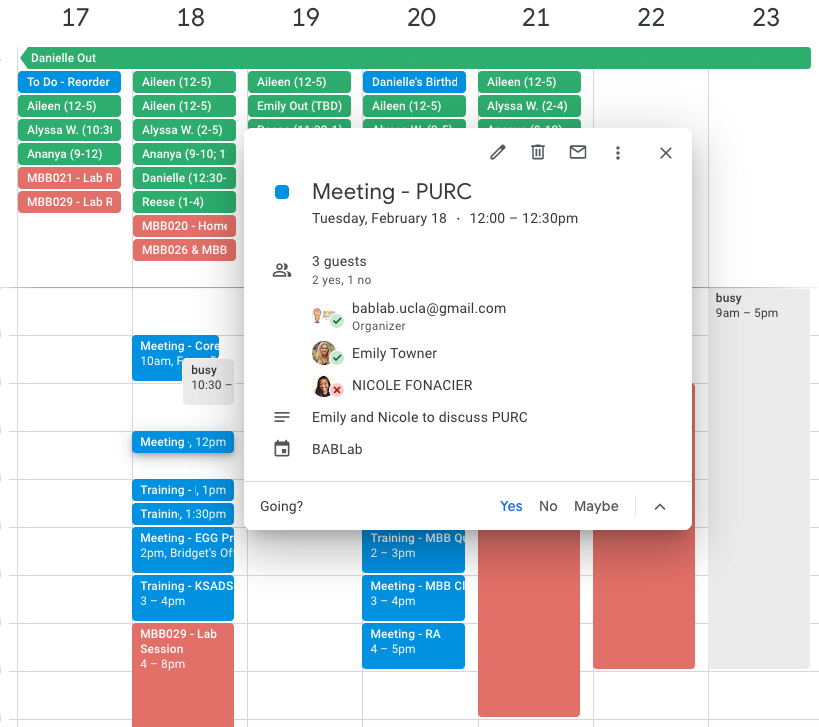
\includegraphics{images/lab_protocols/trainee_tuesdays_thursdays/1.png}
\caption{}
\end{figure}

I (Emily) have also shared my personal calendar with the BABLab account, so you can see when I am available to meet with you. You can access it by selecting ``Emily Towner'' from ``Other calendars'' in the BABLab calendar. The off-white ``busy'' slots are times I am unavailable (doctor's appointments, non lab-related meetings etc.).

\begin{figure}
\centering
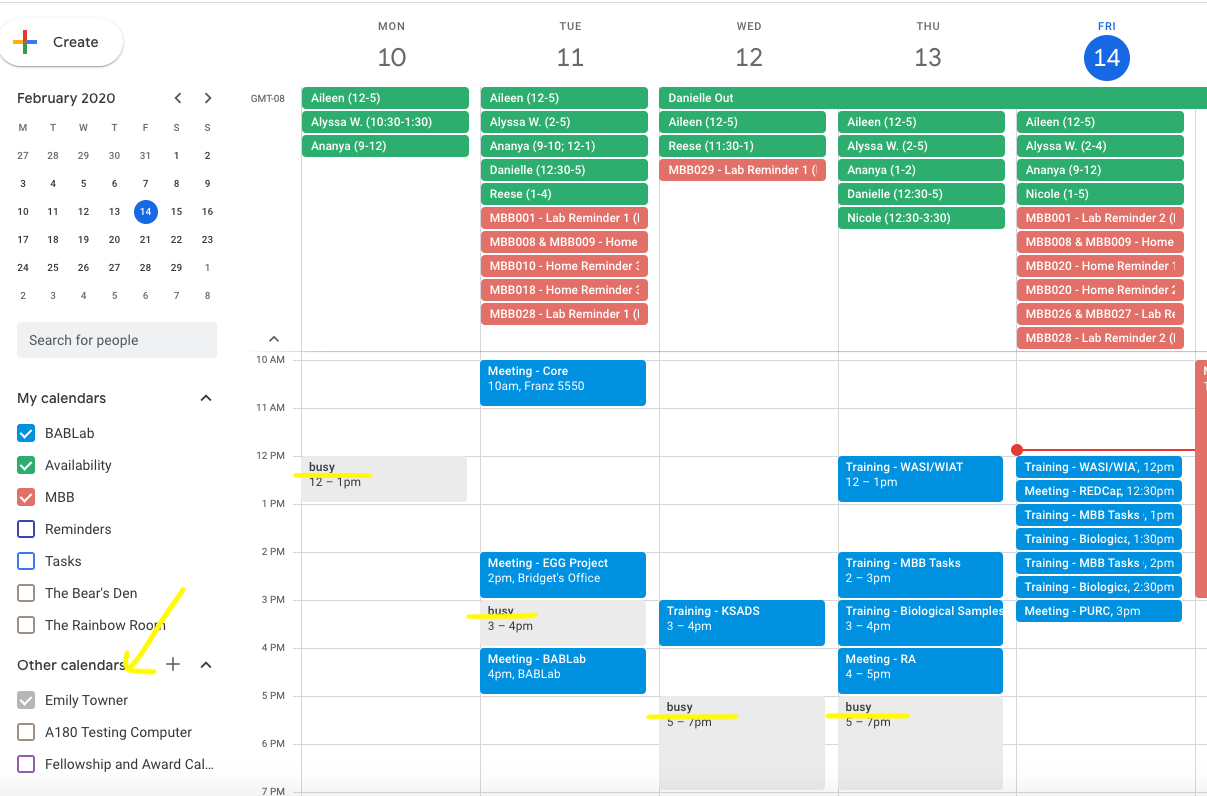
\includegraphics{images/lab_protocols/trainee_tuesdays_thursdays/2.png}
\caption{}
\end{figure}

\begin{center}\rule{0.5\linewidth}{0.5pt}\end{center}

\hypertarget{clinical-meetings}{%
\subsection{Clinical Meetings}\label{clinical-meetings}}

Purpose

The purpose of clinical meetings are to discuss and review ongoing clinical interviews (KSADs), troubleshoot any recent difficulties, and learn helpful interviewing tactics for future clinical interviews. During the meeting, you will present the team with background information from your clinical interview and walk through each supplement.

What To Prepare

Using a shared Dropbox Paper document, please prepare the following:

\begin{itemize}
\tightlist
\item
  Who you are presenting

  \begin{itemize}
  \tightlist
  \item
    Participant's KSADS file
  \item
    Date/time of session
  \end{itemize}
\item
  Brief background

  \begin{itemize}
  \tightlist
  \item
    Was the child bio/adopted?

    \begin{itemize}
    \tightlist
    \item
      Age of adoption
    \end{itemize}
  \item
    Was there any prenatal exposure?
  \item
    Any trouble in school?
  \end{itemize}
\item
  Supplements

  \begin{itemize}
  \tightlist
  \item
    Your thought process on why/why not you went through each supplements/diagnoses you have assigned
  \end{itemize}
\item
  Personal opinions

  \begin{itemize}
  \tightlist
  \item
    What was the child participant like in the session? (note relevant behaviors for context)
  \end{itemize}
\item
  WASI/WIAT

  \begin{itemize}
  \tightlist
  \item
    A quick overview of the participant's WASI/WIAT (admission and scores)
  \end{itemize}
\item
  Questions for the team

  \begin{itemize}
  \tightlist
  \item
    Any situations you feel may have been difficult to address during the clinical interview
  \end{itemize}
\end{itemize}

\emph{These meetings are also a safe space to debrief potentially difficult interviews.}

\begin{center}\rule{0.5\linewidth}{0.5pt}\end{center}

\hypertarget{mail}{%
\section{Mail}\label{mail}}

\begin{center}\rule{0.5\linewidth}{0.5pt}\end{center}

\hypertarget{usps}{%
\subsection{USPS}\label{usps}}

When sending things out USPS, you can place your recharge ID under the sender's address, circle it, \& drop it in the outgoing mail bin in 1282 (faculty mailroom)

\begin{center}\rule{0.5\linewidth}{0.5pt}\end{center}

\hypertarget{recycling-waste}{%
\section{Recycling \& Waste}\label{recycling-waste}}

We can leave small items outside our door for recycling/trash pickup. For large items we should bring them to the A-level loading dock to be recycled.

\begin{center}\rule{0.5\linewidth}{0.5pt}\end{center}

\hypertarget{purchasing}{%
\section{Purchasing}\label{purchasing}}

\begin{center}\rule{0.5\linewidth}{0.5pt}\end{center}

\hypertarget{pac-orders}{%
\subsection{PAC Orders}\label{pac-orders}}

PAC forms are used for most purchasing requests (besides Amazon which we can order from directly with our Amazon business account). Please consult the \href{http://staff.purchasing.ucla.edu/Portal/app/agreements/agreementsummary.aspx}{UCLA preferred vendors list} first before submitting a PAC form for an outside vendor.

\begin{itemize}
\tightlist
\item
  Save any quote to (BABLAB/Lab/Finances/Purchasing/)
\item
  Check Trello purchasing board for existing item
\item
  If no existing item, create one and add description based on templates
\item
  Fill out blank PAC form located in (BABLAB/Lab/Lab\_protocols/Finances/Purchasing/)
\item
  Save to (BABLAB/Lab/Finances/Purchasing)
\item
  Email the completed PAC order form to \href{mailto:psych-orders@psych.ucla.edu}{\nolinkurl{psych-orders@psych.ucla.edu}}

  \begin{itemize}
  \tightlist
  \item
    \textbf{Subject} - CB, {[}Fill in Vendor{]} Request, Bridget Callaghan
  \item
    CC' Bridget (\href{mailto:bcallaghan@ucla.edu}{\nolinkurl{bcallaghan@ucla.edu}}) - do not need signature if PI is cc'd
  \end{itemize}
\item
  Complete item order information on Trello purchasing board
\item
  Save PO (purchase order) and CONF (confirmation) if received
\item
  Once item is received lab manager log amount in funds spreadsheet

  \begin{itemize}
  \tightlist
  \item
    Add in any tax/shipping/expense that wasn't accounted for on Trello to most expensive item
  \item
    Mark as ``Logged'' on Trello
  \end{itemize}
\end{itemize}

\begin{center}\rule{0.5\linewidth}{0.5pt}\end{center}

\hypertarget{amazon-orders}{%
\subsection{Amazon Orders}\label{amazon-orders}}

Instructions for checking out via our Amazon Business Account.

\begin{itemize}
\tightlist
\item
  Check for existing item on Trello
\item
  If existing item, move to ``To Order'' list, change label to not logged, and create new instance of purchase in description box
\item
  To checkout via Amazon, Choose a Group

  \begin{itemize}
  \tightlist
  \item
    Upon clicking ``Proceed to Checkout'' you will arrive to the screen below. Select your fund manager's group and click continue:
  \item
    Be sure to select the correct group to avoid your order being rejected or sitting in a queue that is not being reviewed. In the event that your fund manager is out of the office, please check with the Business Office before starting your Amazon Business order so that we can add you to another group temporarily. Otherwise, the order will remain in your fund manager's queue until they are back in the office and able to approve orders.
  \end{itemize}
\item
  Business Order Information

  \begin{itemize}
  \tightlist
  \item
    Enter the Full Accounting Unit (FAU) or Recharge ID in the Purchase Order (PO) Number field and enter a business justification in the Comments for Approver field. These fields are required for the Psychology Department. If this information is not provided, your fund manager will reject the order.
  \item
    NOTE: Business justifications must describe the purpose of items being purchased, how and where the items will be used. Please be sure to be as detailed and specific as possible. If you are purchasing an item flagged as restricted your fund manager may reach out to you for additional information.\\
  \item
    Restricted items are not necessarily unallowable, but may require additional levels of approval from the Pcard Administrator in Purchasing before we can charge it to a Pcard.
  \end{itemize}
\item
  Next, select the appropriate shipping address
\item
  Next, you will select the method of payment. This should be a VISA with your fund manager's name on the card. You do not have the option to edit this page and it is not necessary to include a reference number. Click continue.
\item
  Review your order details and once confirmed, click on submit order for approval.
\item
  Complete item order information on Trello and move to ``Submitted'' list
\item
  Once placed, move item to ``Placed'' list on Trello
\item
  Once item is received, lab manager to log amount in funds spreadsheet

  \begin{itemize}
  \tightlist
  \item
    Add in any tax/shipping/expense that wasn't accounted for on Trello to most expensive item
  \item
    Mark as ``Logged'' on Trello
  \end{itemize}
\end{itemize}

\begin{center}\rule{0.5\linewidth}{0.5pt}\end{center}

\hypertarget{reimbursement}{%
\subsection{Reimbursement}\label{reimbursement}}

For reimbursement:

\begin{itemize}
\tightlist
\item
  Fill out a blank reimbursement form found in (BABLAB/Lab/Lab\_protocols/Finances/Reimbursement/)
\item
  Save reimbursement form to (BABLAB/Lab/Finances/Reimbursement)
\item
  Email the completed reimbursement form to \href{mailto:psych-orders@psych.ucla.edu}{\nolinkurl{psych-orders@psych.ucla.edu}}

  \begin{itemize}
  \tightlist
  \item
    Subject - CB, {[}Fill in Vendor{]} Reimbursement, Bridget Callaghan
  \item
    CC' Bridget (\href{mailto:bcallaghan@ucla.edu}{\nolinkurl{bcallaghan@ucla.edu}}) - do not need signature if PI is cc'd
  \end{itemize}
\item
  Lab manager log reimbursement amount in funds spreadsheet
\end{itemize}

\begin{center}\rule{0.5\linewidth}{0.5pt}\end{center}

\hypertarget{guest-parking-passes}{%
\subsection{Guest Parking Passes}\label{guest-parking-passes}}

\begin{itemize}
\tightlist
\item
  Email Tyler Tuione (\href{mailto:tuione@psych.ucla.edu}{\nolinkurl{tuione@psych.ucla.edu}}) saying you would like to purchase guest parking passes.
\item
  Information to include in this email:

  \begin{itemize}
  \tightlist
  \item
    Number of passes to order
  \item
    Recharge ID for fund to charge
  \end{itemize}
\item
  Wait for Parking Services to call the lab (about a week), record the confirmation code they give you.
\item
  Pick up the passes with the confirmation code at 555 Westwood Plaza, Suite 100.
\end{itemize}

\begin{center}\rule{0.5\linewidth}{0.5pt}\end{center}

\hypertarget{petty-cash}{%
\subsection{Petty Cash}\label{petty-cash}}

\begin{itemize}
\tightlist
\item
  Fill out a blank IRB research payment request form (for cash or card)(BABLAB/Lab/Lab\_protocols/Finances/Petty\_cash/)
\item
  Send it to Brian Hoang (\href{mailto:brianhoang@psych.ucla.edu}{\nolinkurl{brianhoang@psych.ucla.edu}}) for a signature
\item
  Submit the form at this \href{https://sa.ucla.edu/MessageCenter/OneStop/Home/PostMessage?topicId=293}{site}
\item
  It can take up to 10 business days for them to reply back.
\item
  When they recontact with a delivery time, ensure that either of the people who signed the form (Bridget and an RA) are in the lab at the time of delivery to sign off on the order.
\item
  They will not deliver the cash if one of the signers is not present
\item
  Once the disbursement is received, log it on the study specific payment log
\item
  Ask the lab manager to log the pettycash amount in the funds spreadsheet
\end{itemize}

\begin{center}\rule{0.5\linewidth}{0.5pt}\end{center}

\hypertarget{vendor-specific-protocols}{%
\subsection{Vendor specific protocols}\label{vendor-specific-protocols}}

Some vendors have special requirements or instructions to make purchases from them.

Biopac
- Email \href{mailto:aimeew@biopac.com}{\nolinkurl{aimeew@biopac.com}} and \href{mailto:frontdesk@biopac.com}{\nolinkurl{frontdesk@biopac.com}}

Uprinting

\begin{itemize}
\tightlist
\item
  Go to Uprinting.com and log in.
\item
  Select the items you want to purchase and add them to the cart.

  \begin{itemize}
  \tightlist
  \item
    Note that you need to have the pdf or image files on-hand and make sure they match the dimensions of what they will be printed on
  \end{itemize}
\item
  When checking out, select ``Terms'' as the payment method
\item
  Create and submit a PAC form to purchasing as usual, but also cc' \href{mailto:jhoan.e@digitalroominc.com}{\nolinkurl{jhoan.e@digitalroominc.com}} and request that purchasing get in touch with her to pay for the order
\end{itemize}

\begin{center}\rule{0.5\linewidth}{0.5pt}\end{center}

\hypertarget{logging-purchases-on-trello}{%
\subsection{Logging purchases on Trello}\label{logging-purchases-on-trello}}

\begin{enumerate}
\def\labelenumi{\arabic{enumi}.}
\tightlist
\item
  Go to the ``Purchasing'' board on Trello. It should be green.There are different tabs:
\end{enumerate}

\begin{itemize}
\tightlist
\item
  \textbf{To Return}: items that will be returned
\item
  \textbf{Maybe}: items that may be bought
\item
  \textbf{To Order}: items to order/ buy
\item
  \textbf{Submitted}: orders that have been submitted
\item
  \textbf{Placed}: orders that have been placed
\item
  \textbf{In Stock}: items that have arrived and are in lab
\end{itemize}

\begin{enumerate}
\def\labelenumi{\arabic{enumi}.}
\setcounter{enumi}{1}
\item
  Add a card to ``To Order'' - name it with this format: \textbf{item being bought - \$price}
\item
  Add the following labels:
\end{enumerate}

\begin{itemize}
\tightlist
\item
  \textbf{Budget: Nonlogged} (always log this by default)
\item
  \textbf{Fund} (ask lab manager whether it's Startup, R00, or other fund)
\item
  \textbf{Category} (ask lab manager which category)
\end{itemize}

\begin{enumerate}
\def\labelenumi{\arabic{enumi}.}
\setcounter{enumi}{3}
\item
  Add the link of the item on `add an attachment'. Rename the link the exact name of the item as written on Amazon (or whatever website).
\item
  Add a description with this format:
\end{enumerate}

\begin{itemize}
\tightlist
\item
  Units: (insert amount of item, ex. 20 pencils)
\item
  Orders: (insert how many orders placed, ex. 1 order of 20 pencils)
\item
  Date submitted: (insert date we submitted order)
\item
  Date placed: (insert date vendor has placed order)
\item
  Date received: (insert date we got it in lab)
\item
  If the card is something that may run out eventually (ex. granola bars, notebooks) add an approximate due date.
\end{itemize}

\begin{enumerate}
\def\labelenumi{\arabic{enumi}.}
\setcounter{enumi}{5}
\tightlist
\item
  Whenever an item has been submitted, placed, and in stock, move the card into its respective tab.
\end{enumerate}

Watch the video for a detailed explanation.

\begin{center}\rule{0.5\linewidth}{0.5pt}\end{center}

\hypertarget{technology}{%
\section{Technology}\label{technology}}

\begin{center}\rule{0.5\linewidth}{0.5pt}\end{center}

\hypertarget{slack}{%
\subsection{Slack}\label{slack}}

If you haven't already found this out for yourself, emails are a clunky way of communicating for most lab needs. Moreover, most people will find that they have a backlog of emails awaiting their attention. For this reason, we will use Slack for the primary means of lab communication.

The beauty of Slack is that you only subscribe to the channels that concern you. For messages to one person or a small group, use direct messages. If you have to include out-of-lab recipients, use e-mail. If you have a paper you want to share, download it and then upload it to Slack in the \#papers channel.

Full-time lab members should install Slack on their computers and/or phones and check it regularly (during working hours). Part-time lab members should also check Slack when they are working in the lab as there may be important messages in there for them.

Of course, if there is an emergency, and you need to contact Bridget, use her email or phone or drop into her office.

\begin{longtable}[]{@{}lll@{}}
\toprule
\begin{minipage}[b]{0.18\columnwidth}\raggedright
Slack Channel\strut
\end{minipage} & \begin{minipage}[b]{0.04\columnwidth}\raggedright
Type\strut
\end{minipage} & \begin{minipage}[b]{0.70\columnwidth}\raggedright
Purpose\strut
\end{minipage}\tabularnewline
\midrule
\endhead
\begin{minipage}[t]{0.18\columnwidth}\raggedright
\#bablab\_core\strut
\end{minipage} & \begin{minipage}[t]{0.04\columnwidth}\raggedright
Private\strut
\end{minipage} & \begin{minipage}[t]{0.70\columnwidth}\raggedright
For private communication between the core team - this includes the PI, Lab Managers, Postdocs, and Grad Students\strut
\end{minipage}\tabularnewline
\begin{minipage}[t]{0.18\columnwidth}\raggedright
\#bablab\_ra\strut
\end{minipage} & \begin{minipage}[t]{0.04\columnwidth}\raggedright
Private\strut
\end{minipage} & \begin{minipage}[t]{0.70\columnwidth}\raggedright
For private communication between the lab managers and all the research assistants\strut
\end{minipage}\tabularnewline
\begin{minipage}[t]{0.18\columnwidth}\raggedright
\#bablab\_senior\_ra\strut
\end{minipage} & \begin{minipage}[t]{0.04\columnwidth}\raggedright
Private\strut
\end{minipage} & \begin{minipage}[t]{0.70\columnwidth}\raggedright
For private communication between the lab managers and the senior research assistants\strut
\end{minipage}\tabularnewline
\begin{minipage}[t]{0.18\columnwidth}\raggedright
\#general\strut
\end{minipage} & \begin{minipage}[t]{0.04\columnwidth}\raggedright
Public\strut
\end{minipage} & \begin{minipage}[t]{0.70\columnwidth}\raggedright
For lab-wide communication and announcements\strut
\end{minipage}\tabularnewline
\begin{minipage}[t]{0.18\columnwidth}\raggedright
\#meetings\_lab\strut
\end{minipage} & \begin{minipage}[t]{0.04\columnwidth}\raggedright
Public\strut
\end{minipage} & \begin{minipage}[t]{0.70\columnwidth}\raggedright
For notes or communication related to lab meetings\strut
\end{minipage}\tabularnewline
\begin{minipage}[t]{0.18\columnwidth}\raggedright
\#methods\_fmri\strut
\end{minipage} & \begin{minipage}[t]{0.04\columnwidth}\raggedright
Public\strut
\end{minipage} & \begin{minipage}[t]{0.70\columnwidth}\raggedright
Sharing wisdom on fMRI data collection / analysis or asking (and answering) the fMRI questions of others\strut
\end{minipage}\tabularnewline
\begin{minipage}[t]{0.18\columnwidth}\raggedright
\#methods\_mb\strut
\end{minipage} & \begin{minipage}[t]{0.04\columnwidth}\raggedright
Public\strut
\end{minipage} & \begin{minipage}[t]{0.70\columnwidth}\raggedright
Sharing wisdom on microbiome data collection / analysis or asking and answering the microbiome questions of others\strut
\end{minipage}\tabularnewline
\begin{minipage}[t]{0.18\columnwidth}\raggedright
\#notes\_conferences\strut
\end{minipage} & \begin{minipage}[t]{0.04\columnwidth}\raggedright
Public\strut
\end{minipage} & \begin{minipage}[t]{0.70\columnwidth}\raggedright
For taking notes at conferences\strut
\end{minipage}\tabularnewline
\begin{minipage}[t]{0.18\columnwidth}\raggedright
\#papers\strut
\end{minipage} & \begin{minipage}[t]{0.04\columnwidth}\raggedright
Public\strut
\end{minipage} & \begin{minipage}[t]{0.70\columnwidth}\raggedright
Sharing links to lab-relevant papers and discussing them\strut
\end{minipage}\tabularnewline
\begin{minipage}[t]{0.18\columnwidth}\raggedright
\#random\strut
\end{minipage} & \begin{minipage}[t]{0.04\columnwidth}\raggedright
Public\strut
\end{minipage} & \begin{minipage}[t]{0.70\columnwidth}\raggedright
Non-work-related chatting -- e.g., pics of pets, funny cartoons etc.\strut
\end{minipage}\tabularnewline
\begin{minipage}[t]{0.18\columnwidth}\raggedright
\#recruitment\strut
\end{minipage} & \begin{minipage}[t]{0.04\columnwidth}\raggedright
Public\strut
\end{minipage} & \begin{minipage}[t]{0.70\columnwidth}\raggedright
Any ideas you have for recruiting youth into our study\strut
\end{minipage}\tabularnewline
\begin{minipage}[t]{0.18\columnwidth}\raggedright
\#stats\strut
\end{minipage} & \begin{minipage}[t]{0.04\columnwidth}\raggedright
Public\strut
\end{minipage} & \begin{minipage}[t]{0.70\columnwidth}\raggedright
To ask and answer questions about statistical analyses\strut
\end{minipage}\tabularnewline
\begin{minipage}[t]{0.18\columnwidth}\raggedright
\#study\_egg\_emotionality\strut
\end{minipage} & \begin{minipage}[t]{0.04\columnwidth}\raggedright
Private\strut
\end{minipage} & \begin{minipage}[t]{0.70\columnwidth}\raggedright
To discuss issues related to the EGG and Emotionality study\strut
\end{minipage}\tabularnewline
\begin{minipage}[t]{0.18\columnwidth}\raggedright
\#study\_mbb\strut
\end{minipage} & \begin{minipage}[t]{0.04\columnwidth}\raggedright
Private\strut
\end{minipage} & \begin{minipage}[t]{0.70\columnwidth}\raggedright
To discuss issues related to the Mind, Brain, Body study\strut
\end{minipage}\tabularnewline
\begin{minipage}[t]{0.18\columnwidth}\raggedright
\#study\_transfer\_mental\_health\strut
\end{minipage} & \begin{minipage}[t]{0.04\columnwidth}\raggedright
Private\strut
\end{minipage} & \begin{minipage}[t]{0.70\columnwidth}\raggedright
To discuss issues related to the Transfer Mental Health Study\strut
\end{minipage}\tabularnewline
\begin{minipage}[t]{0.18\columnwidth}\raggedright
\#tips\_coding\strut
\end{minipage} & \begin{minipage}[t]{0.04\columnwidth}\raggedright
Public\strut
\end{minipage} & \begin{minipage}[t]{0.70\columnwidth}\raggedright
Sharing wisdom on code writing or asking (and answering) the coding questions of others\strut
\end{minipage}\tabularnewline
\bottomrule
\end{longtable}

\begin{center}\rule{0.5\linewidth}{0.5pt}\end{center}

\hypertarget{box}{%
\subsection{Box}\label{box}}

We have moved over to Box for our file storage service. This works very similarly to Google Drive or Dropbox, but is more secure. Additionally, each lab member can have their own account, it's free and great for collaboration!

Please download \href{https://www.box.com/drive}{Box Drive} to use.

\begin{enumerate}
\def\labelenumi{\arabic{enumi}.}
\tightlist
\item
  Click download for your operating system
\end{enumerate}

\begin{figure}
\centering
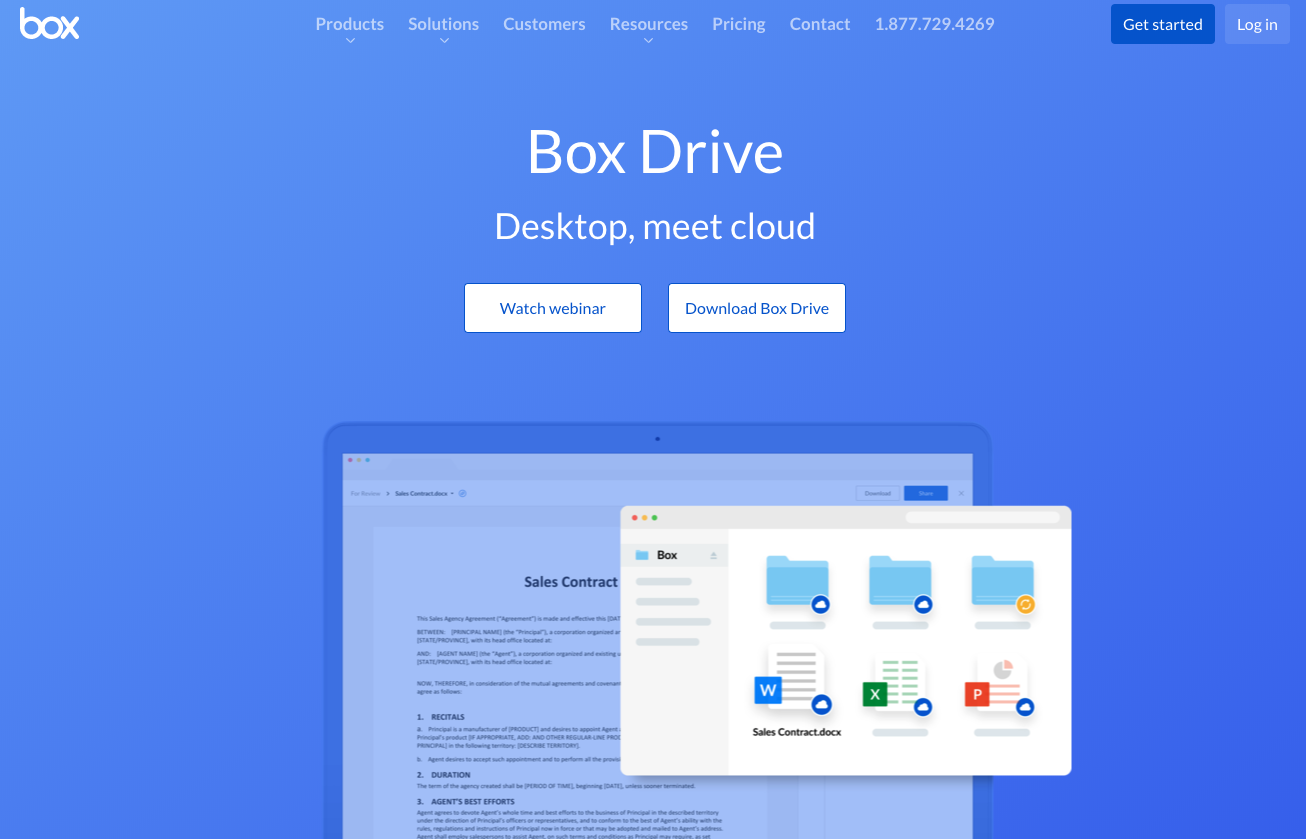
\includegraphics{images/lab_protocols/box/1.png}
\caption{}
\end{figure}

\begin{enumerate}
\def\labelenumi{\arabic{enumi}.}
\setcounter{enumi}{1}
\tightlist
\item
  After installing, you may need to click allow in your security preferences
\end{enumerate}

\begin{figure}
\centering
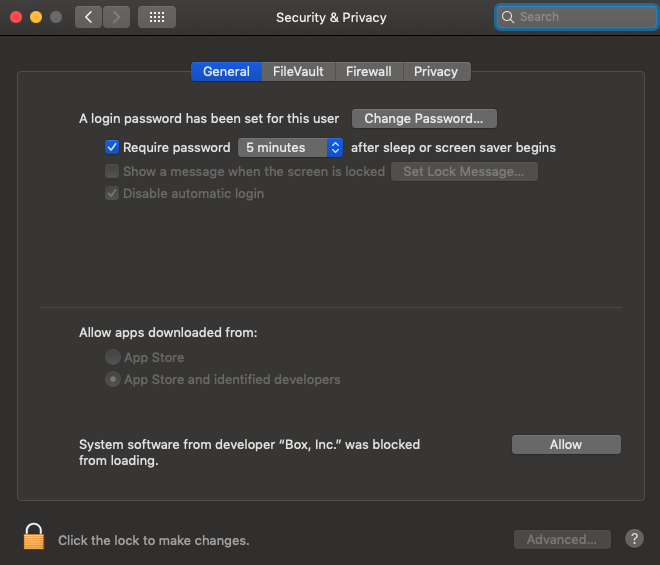
\includegraphics{images/lab_protocols/box/2.png}
\caption{}
\end{figure}

\begin{enumerate}
\def\labelenumi{\arabic{enumi}.}
\setcounter{enumi}{2}
\tightlist
\item
  Log in with your UCLA email (make sure to accept the Box sharing request first)
\end{enumerate}

\begin{figure}
\centering
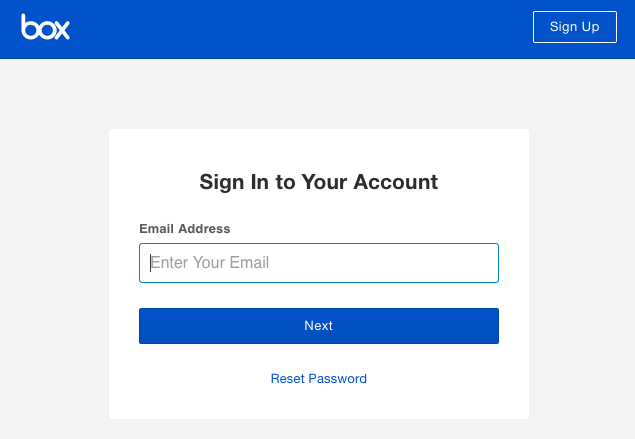
\includegraphics{images/lab_protocols/box/3.png}
\caption{}
\end{figure}

\begin{enumerate}
\def\labelenumi{\arabic{enumi}.}
\setcounter{enumi}{3}
\tightlist
\item
  Now you can use Box on your desktop.
\end{enumerate}

\begin{figure}
\centering
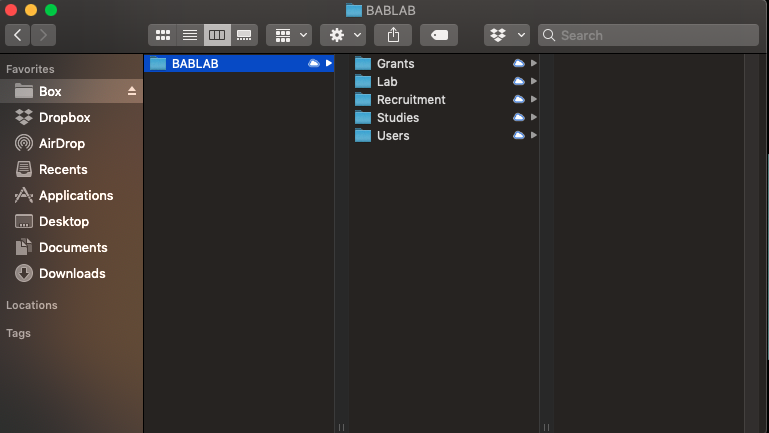
\includegraphics{images/lab_protocols/box/4.png}
\caption{}
\end{figure}

\begin{enumerate}
\def\labelenumi{\arabic{enumi}.}
\setcounter{enumi}{4}
\tightlist
\item
  On the web version, change your notification preferences so that you don't get an email every time someone uploads a file by unchecking the boxes below
\end{enumerate}

\begin{figure}
\centering
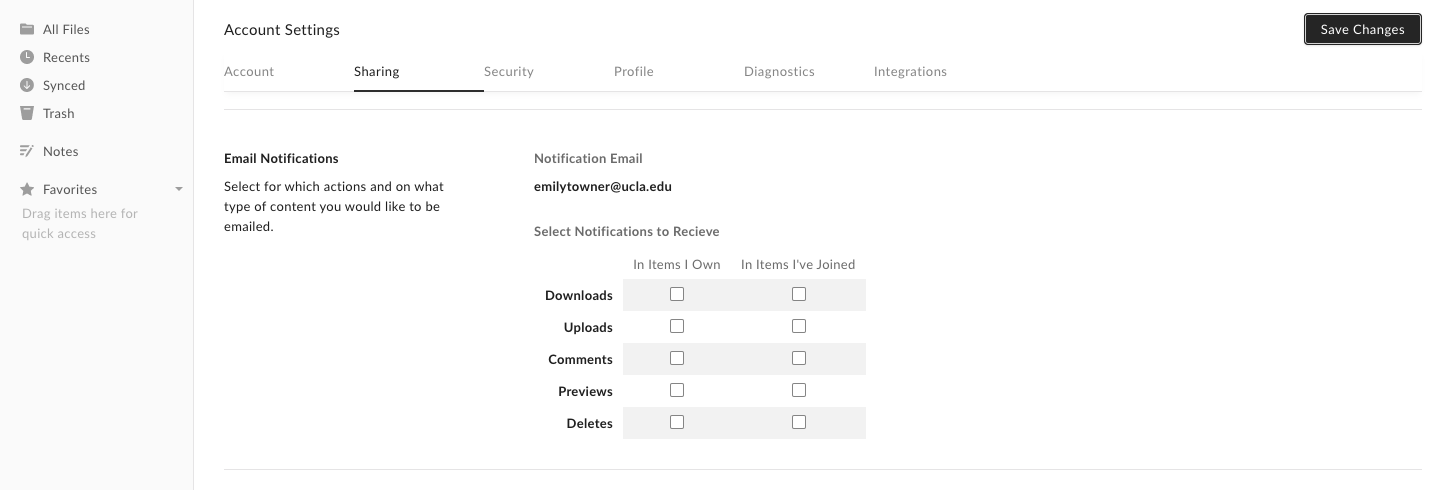
\includegraphics{images/lab_protocols/box/5.png}
\caption{}
\end{figure}

\begin{center}\rule{0.5\linewidth}{0.5pt}\end{center}

\hypertarget{using-trello}{%
\subsection{Using Trello}\label{using-trello}}

\begin{enumerate}
\def\labelenumi{\arabic{enumi}.}
\tightlist
\item
  There are multiple lists on the Tasks Board!
  These include: Doing, To-do, Later and Done.
  Depending on the task, simply move it to the right list once you progress with it.
\end{enumerate}

\begin{itemize}
\tightlist
\item
  \textbf{To Do:} Current tasks to complete.
\item
  \textbf{Doing:} Tasks currently being done.
\item
  \textbf{Later}: Tasks not as pressing, but still must be done.
\item
  \textbf{Done}: Completed tasks.
\end{itemize}

\begin{enumerate}
\def\labelenumi{\arabic{enumi}.}
\setcounter{enumi}{1}
\tightlist
\item
  \textbf{To add a card}: Click `+ Add Another Card' under the appropriate list. There are multiple functions within this:
\end{enumerate}

\begin{itemize}
\tightlist
\item
  You can add members, labels (useful for studies), checklist, attachment, due date and more to the back of the card. This information will show when you click on the card.
\end{itemize}

\begin{enumerate}
\def\labelenumi{\arabic{enumi}.}
\setcounter{enumi}{2}
\tightlist
\item
  \textbf{Show Menu function:} This is a great way to search specific items, such as your own name for tasks, or the study for which there are tasks for, or tasks which have upcoming due dates.
\end{enumerate}

\begin{center}\rule{0.5\linewidth}{0.5pt}\end{center}

\hypertarget{server}{%
\subsection{Server}\label{server}}

In addition to Box, we make regular biweekly backups to a dedicated psychology department server (in addition to two external drives)

To connect to the CallaghanLab server:

*Contact the lab manager first to set up your credentials.

On a Mac --

\begin{itemize}
\tightlist
\item
  From the dropdown menu under ``Go'', select ``Connect to Server\ldots{}'' (Apple + K)
\item
  Enter the network/server address: \texttt{smb://pythia.psych.ucla.edu/Users/CallaghanLab/}
\item
  Click on ``Connect''.
\item
  A dialogue box will prompt you for your credentials. Enter your credentials obtained from Psychology IT and click on ``OK''.
\item
  If everything was entered correctly from above, the mapped drive will appear under ``Shared'' in the Mac's Finder.
\end{itemize}

On a PC --

\begin{itemize}
\tightlist
\item
  From the Windows file explorer, right mouse click on ``Computer'' for Windows 7 or ``This PC'' on Windows 8/10.
\item
  Select ``Map network drive''.
\item
  Specify an available ``Drive'' letter from the dropdown menu.
\item
  Enter the network/server location for the ``Folder'' field and click on ``Finish''.

  \begin{itemize}
  \tightlist
  \item
    Network/server location: \texttt{\textbackslash{}\textbackslash{}pythia.psych.ucla.edu\textbackslash{}Users\textbackslash{}CallaghanLab\textbackslash{}}
  \end{itemize}
\item
  Enter your username and password that was provided by Psychology IT in the ``network credentials'' popup dialogue box and click on OK.
\item
  If everything was entered correctly from above, the mapped drive will appear under ``Network locations'' when you click on ``Computer/This PC''.
\item
  After the drive has been mapped, logged out of Windows to ``logout'' from the network drive.
\item
  Don't right mouse click on the mapped drive and select ``Disconnect''. This will only unmap the network drive and you will have to go through the process all over again.
\end{itemize}

To connect off-campus connect to the UCLA/BOL VPN and let it run in the background prior to logging into the mapped drive you had configured on your computer.

How-to download/install the \href{https://help.bol.ucla.edu/kb_view.do?sysparm_article=kb0010923}{Cisco VPN client}.

\begin{quote}
Every night the server is backed up to the Life Sciences data center in Hershey Hall. That's always been the case. To make those nightly backups more safe, there is another copy of the backups stored offsite (i.e.~to prevent losing both the server AND the backups in a fire, earthquake, etc.)

Once we have Shadow Copy enabled, we'll also have more direct access to backups, so we won't need to work with Life Sciences to retrieve backups. Psych IT will be able to grab a recent copy of your files/folders ourselves. We'll also have access to incremental backups (i.e.~yesterday's copy, two day old copy, three day old copy\ldots{}up to two weeks back).

So at that point we'll have 3 forms of backup, and plenty of safety net.

\begin{itemize}
\tightlist
\item
  Dave (Psych IT)
\end{itemize}
\end{quote}

\begin{center}\rule{0.5\linewidth}{0.5pt}\end{center}

\hypertarget{dropbox-paper}{%
\subsection{Dropbox Paper}\label{dropbox-paper}}

The lab has a shared Dropbox Paper account --- which is slightly different than regular Dropbox file storage. On the Dropbox Paper, we will place collaborative documents. We will grant you access permission to various folders in the Dropbox Paper account, You may need to initialize an account with the email we grant access permission.

\begin{center}\rule{0.5\linewidth}{0.5pt}\end{center}

\hypertarget{github}{%
\subsection{GitHub}\label{github}}

The lab's GitHub should be used to share code and data with people outside of the lab (i.e., people not on our IRB). Not all data can be shared (because of IRB restrictions) and not all data that can be shared should be shared immediately. Speak with Bridget about when to share data, and what needs to be done to the data (e.g., the level of de-identification required) before we share it. Ask the lab manager to get access to the lab's GitHub.

Our lab manual, lab wiki, and study wikis are also hosted on our GitHub.

\begin{center}\rule{0.5\linewidth}{0.5pt}\end{center}

\hypertarget{google-calendars}{%
\subsection{Google Calendars}\label{google-calendars}}

The lab has many Google calendars and you should subscribe to those that make sense for your unique situation.

\begin{enumerate}
\def\labelenumi{\arabic{enumi}.}
\tightlist
\item
  \textbf{BABLab:} Used for lab meetings, out of schedule meetings, birthdays, formal lab events etc.
\item
  \textbf{Availability:} If you are part time, please place the hours you plan to come into the lab on this calendar. If you are going to be away, please place the dates and times on this calendar. This is critical as the lab manager will use this information when scheduling people to run participants for our studies. Bridget and the core team will also put her out of office times on this calendar to help people with scheduling.\\
\item
  \textbf{MBB:} Used for booking sessions and reminders for the Mind, Brain, Body study
\item
  \textbf{The Bear's Den:} used to reserve time in experimental room 1
\item
  \textbf{The Rainbow Room:} used to reserve time in experimental room 2
\item
  \textbf{A180 Testing Computer:} the SAND Lab room that can be used for blood spots
\item
  \textbf{HPL1333:} The Health Psychology Lab room that can be used for blood spots
\end{enumerate}

\begin{center}\rule{0.5\linewidth}{0.5pt}\end{center}

\hypertarget{e-mail}{%
\subsection{E-mail}\label{e-mail}}

We have an email listserv for communicating with the whole lab and individuals who subscribe to our list - including visitors and students from other labs who attend our meetings, visiting scholars, etc.

The email is: \textbf{\href{mailto:bablab@googlegroups.com}{\nolinkurl{bablab@googlegroups.com}}}

If you are thinking about joining the lab and would like to be notified about upcoming lab meetings, please request to join the listserv.

There is also a lab email account which people use to contact the lab to participate in studies (\href{mailto:bablab.ucla@gmail.com}{\nolinkurl{bablab.ucla@gmail.com}}). This email account will be staffed by the lab manager/s and they will sort the emails in specific folders within the Gmail account. If you are running a study, it is your responsibility to check your study's folder on the lab Gmail every few days and respond to participant inquiries in the ``potential'' participants folder in relation to your study.

\begin{center}\rule{0.5\linewidth}{0.5pt}\end{center}

\hypertarget{mac-os---catalina}{%
\subsection{Mac OS - Catalina}\label{mac-os---catalina}}

If you upgrade your Mac operating system to Catalina, and wish to run tasks on PsychoPy, you must enable the following settings in the image below.

\begin{figure}
\centering
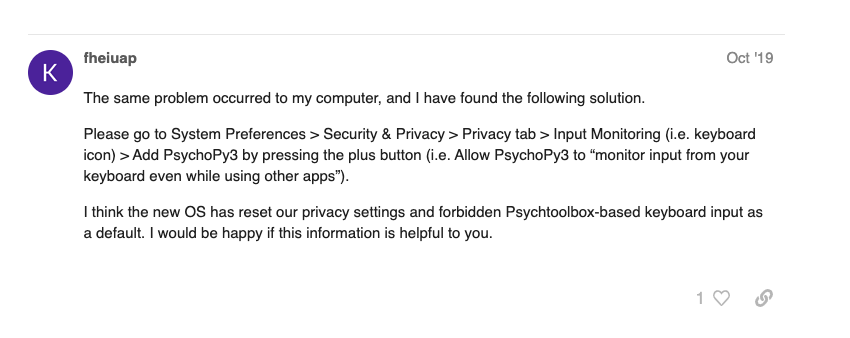
\includegraphics{images/lab_protocols/catalina/1.png}
\caption{}
\end{figure}

\begin{center}\rule{0.5\linewidth}{0.5pt}\end{center}

\hypertarget{redcap}{%
\subsection{REDCap}\label{redcap}}

\hypertarget{entering-instruments}{%
\subsubsection{Entering Instruments}\label{entering-instruments}}

\hypertarget{using-the-test-logic-feature}{%
\subsection{Using the test logic feature}\label{using-the-test-logic-feature}}

You can use the test logic with a record feature to see if this question will be shown for a specific participant

\begin{figure}
\centering
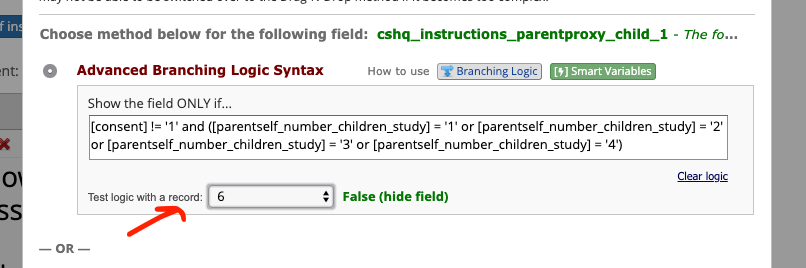
\includegraphics{images/lab_protocols/redcap/1.png}
\caption{}
\end{figure}

\begin{center}\rule{0.5\linewidth}{0.5pt}\end{center}

\hypertarget{r}{%
\subsection{R}\label{r}}

To install R:

\begin{itemize}
\tightlist
\item
  Go to \href{http://www.r-project.org}{R Project}
\item
  Click the ``download R'' link in the middle of the page under ``Getting Started''
\item
  Select a CRAN location (a mirror site) and click the corresponding link
\item
  Click on the ``Download R for (Mac) OS X'' link at the top of the page
\item
  Click on the file containing the latest version of R under ``Files''
\item
  Save the .pkg file, double-click it to open, and follow the installation instructions
\end{itemize}

\begin{center}\rule{0.5\linewidth}{0.5pt}\end{center}

\hypertarget{rstudio}{%
\subsection{RStudio}\label{rstudio}}

To install RStudio:

\begin{itemize}
\tightlist
\item
  Go to \href{http://www.rstudio.com}{RStudio} and click on the ``Download RStudio'' button
\item
  Click on ``Download RStudio Desktop''
\item
  Click on the version recommended for your system, or the latest Mac version, save the .dmg file on your computer, double-click it to open, and then drag and drop it to your applications folder
\end{itemize}

\begin{center}\rule{0.5\linewidth}{0.5pt}\end{center}

\hypertarget{python}{%
\subsection{Python}\label{python}}

To install Python:

\begin{itemize}
\tightlist
\item
  Download the \href{https://www.anaconda.com/distribution/}{Anaconda Distribution}
\item
  Be sure that you download the Python 3.7 version. (Note, this can take upwards of 1-2 hours depending on your internet connection)
\item
  Helpful instructions for these checks can be found on the Anaconda User Guide website: \href{https://docs.anaconda.com/anaconda/user-guide/getting-started/}{``Getting Started''}
\item
  Any issues are most likely due to incorrect installation, which is addressed in the \href{https://docs.anaconda.com/anaconda/user-guide/faq/}{FAQ page}
\end{itemize}

\begin{center}\rule{0.5\linewidth}{0.5pt}\end{center}

\hypertarget{vpn-to-lab-computers}{%
\subsection{VPN to Lab Computers}\label{vpn-to-lab-computers}}

We have set up a VPN on the mac mini in the Bear Den (on the left side of the room).
Because this computer has the Acknowledge software installed on it, and has the USB Key for that program you need to use that computer for processing any physiology data. If you are off campus, you can VPN to the computer using the following steps. NB: you will need to have downloaded Cisco Anyconnect - you can access that by clicking \href{https://www.it.ucla.edu/it-support-center/services/virtual-private-network-vpn-clients}{here}

Step 1. Open Cisco and type `ssl.vpn.ucla.edu' and press `connect'

\begin{figure}
\centering
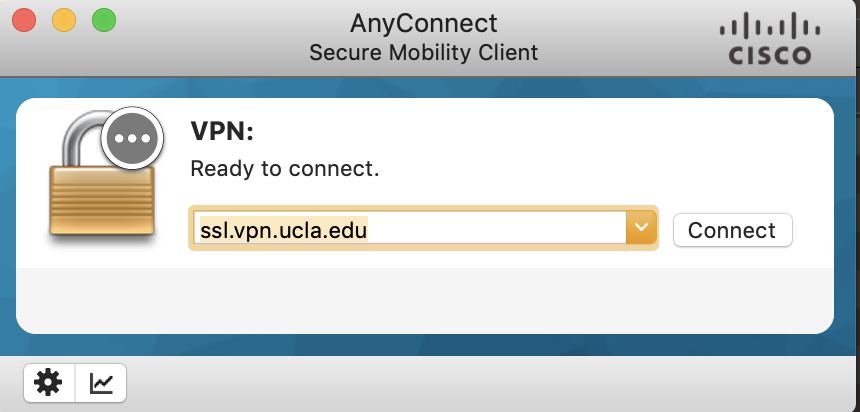
\includegraphics{images/lab_protocols/cisco/1.png}
\caption{}
\end{figure}

Step 2. Type in your UCLA ID and Password (same as you use to get into email)

Step 3. Accept the SSO push to your second device

Step 4. Click `Accept'

Step 5. Go to the magnifying glass at the top right of your screen and search for Screen Sharing.

Step 6. Type in the IP address for the Bear Den computer: 164.67.125.42

Step 7. Type in the username and pw for the Bear Den computer:
Username - Brain \& Body Lab
PW - BaBLaB

Step 8. You will see a new window pop up, with a desktop, which is the desktop of the Bear Den computer.

A second option would be to go to the Finder on your Mac, on the top menu bar click `Go' and then click `Connect to Server'. Type in vpn://164.67.125.42. This will take you straight to the screen sharing page where you can then perform Step 7 \& 8 from above.

\hypertarget{equipment}{%
\section{Equipment}\label{equipment}}

\begin{center}\rule{0.5\linewidth}{0.5pt}\end{center}

\hypertarget{biopac}{%
\subsection{Biopac}\label{biopac}}

\begin{center}\rule{0.5\linewidth}{0.5pt}\end{center}

\hypertarget{printer}{%
\subsection{Printer}\label{printer}}

\begin{itemize}
\tightlist
\item
  Make sure you are connected to eduroam wifi
\item
  Open up Printer \& Scanners in System Preferences

  \begin{itemize}
  \tightlist
  \item
    If current printer is not working, right click printer and click Reset Printing System
    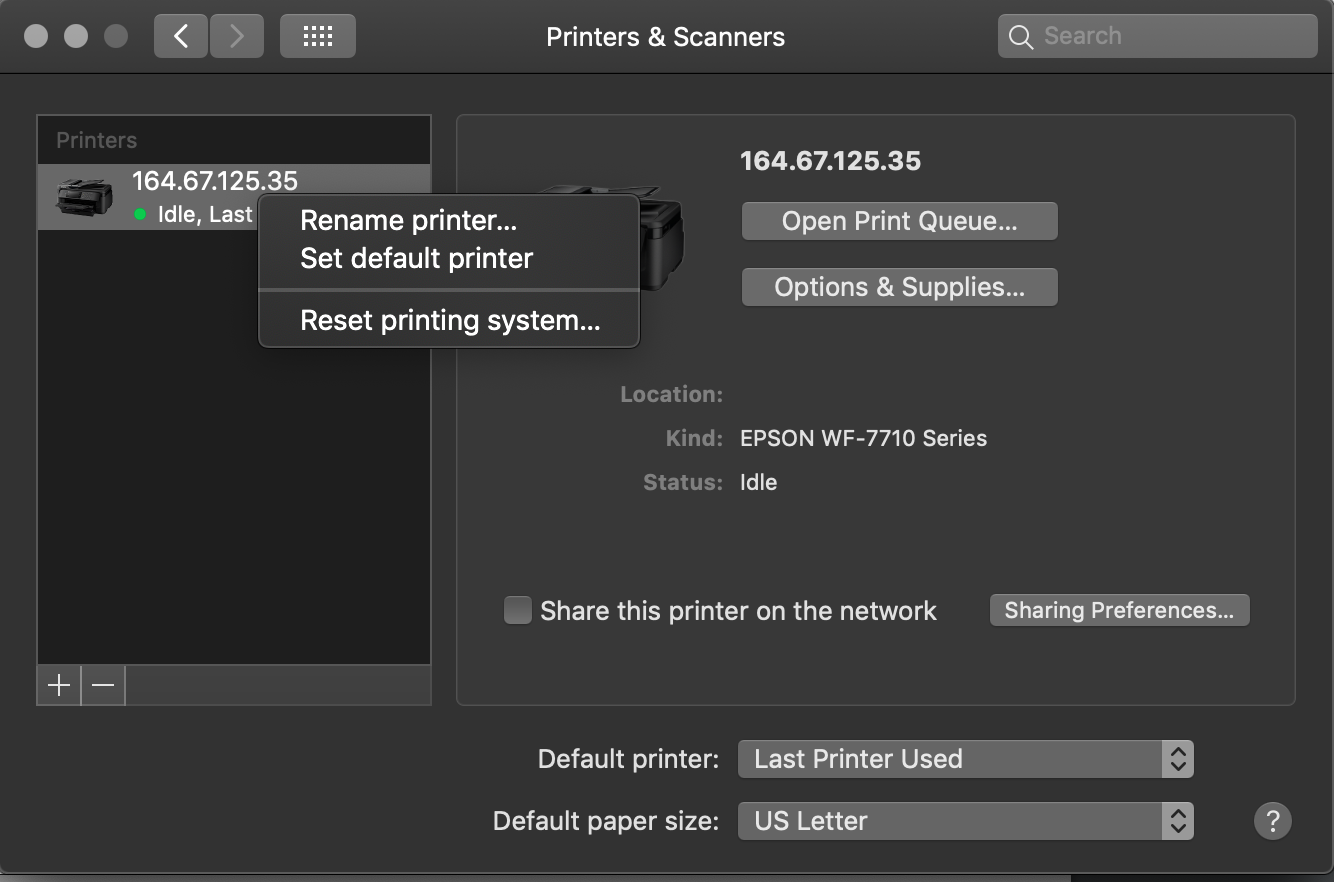
\includegraphics{images/lab_protocols/printer/1.png}
  \end{itemize}
\item
  Reset Computer
\item
  Open up System Preferences -- Printers \& Scanners
\item
  Click on + sign to add a printer
\item
  Enter IP Address from Printer: 164.67.125.35
  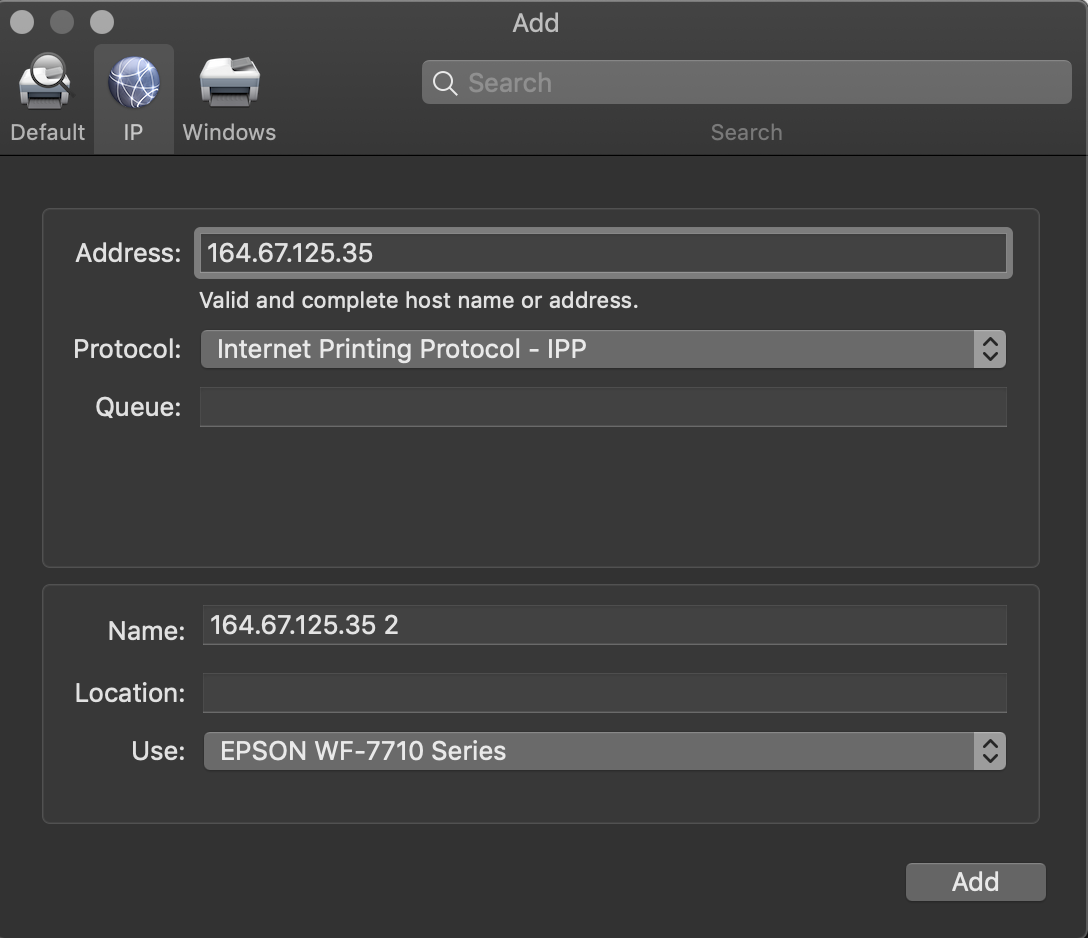
\includegraphics{images/lab_protocols/printer/2.png}
\item
  Make sure Use displays: EPSON WF-7710 Series
\item
  Click ADD
\item
  Reset your Printer Presets if needed
\end{itemize}

\begin{center}\rule{0.5\linewidth}{0.5pt}\end{center}

\hypertarget{social-media}{%
\section{Social Media}\label{social-media}}

\begin{center}\rule{0.5\linewidth}{0.5pt}\end{center}

\hypertarget{instagram}{%
\subsection{Instagram}\label{instagram}}

The pride and joy of the lab. There is a lot of content to keep track of and to ensure is posted weekly.

General important rules:

\begin{itemize}
\tightlist
\item
  Keep posts short, family-friendly, and accessible.
\item
  If you post on the story, it should also likely be added to a story highlight.
\item
  Stick to the color scheme and aesthetic (this includes matching the text in story highlights to the story highlight cover color).
\item
  Maintain the integrity of the main feed grid (will be elaborated on further down).
\item
  Maintain the consistency of the Lab's hashtags (will be elaborated on further down).
\end{itemize}

Feed Content:

\begin{itemize}
\tightlist
\item
  The feed grid is an important part of the aesthetic of the lab's social media. We can divide the grid into ``A Week'' and ``B Week'' rows. Because there are 3 posts horizontally in the grid, there should be 3 pieces of content posted each week (or with relative consistency).
\end{itemize}

``A Week'':

\begin{itemize}
\tightlist
\item
  Biome Bites! ad post: This is simply a post saying to check the story for this week's Biome Bites! installment. The caption for this should be brief and maybe reference the content in the actual story post.
\item
  Lab Meeting ad post OR Email List ad post: Post this on lab meeting day in ``A Week''. If there is a speaker or specific topic for the week, discuss that briefly in the caption.
\item
  In ``B Week'', don't post this even if there is a lab meeting. Instead, post a previous Lab Meeting ad post on the story. If there is not a lab meeting during that ``A Week'', you should post the Email List ad post instead.
\item
  Brain Bites! ad post: This is simply a post saying to check the story for this week's Brain Bites! installment. The caption for this should be brief and maybe reference the content in the actual story post.
\end{itemize}

``B Week'':

\begin{itemize}
\tightlist
\item
  3 random posts: post pictures from around the lab, from events, or advertisements for upcoming events. Check the existing feed for ideas, and try to stay current with seasons, trends, etc.
\item
  If there is an event upcoming, use the following template to advertise it.
\end{itemize}

Important notes for all feed content:

\begin{itemize}
\tightlist
\item
  Post all posts to both instagram and facebook (integrated feature on insta)
\item
  End every single post with the following: \#brain
\item
  Add 2-3 topical hashtags on the new line afterwards, and then follow that with the following block of hashtags: \#funscience \#psychology \#neuroscience \#research \#lablife \#ucla \#gutbiome \#dev \#psych \#brain \#body \#adolescence \#childhood \#ela \#losangeles \#scientist
\end{itemize}

Story Content:

\begin{itemize}
\tightlist
\item
  \textbf{Q\&A Monday:} every Monday, post the Q\&A Monday story with instagram's questions feature attached. Check periodically throughout the day to see if there are any questions worth responding to. Post any responses on the Q\&A story highlight.
\item
  \textbf{Biome Bites!:} A weekly fun fact about the microbiome. Try to stay scientific (with citations) and avoid product/treatment recommendations that might be trendy or controversial. Post the bite itself on the story, and every other week advertise it with a main feed post. Add to the Weekly Bites story highlight.
\item
  \textbf{Lab Meeting ad:} on lab meeting days, post one of the ad posts on the story.
\item
  \textbf{Brain Bites!:} A weekly fun fact about the brain/developmental psych. Try to stay scientific (with citations) and avoid product/treatment recommendations that might be trendy or controversial. Post the bite itself on the story, and every other week advertise it with a main feed post. Add to the Weekly Bites story highlight.
\item
  \textbf{Contact Story ad:} on Fridays, post the contact story post.
\end{itemize}

When events are coming up, be sure to post frequently on the story about the date, time, and what activities we will be doing.

There is a whole series of story templates made to show off different activities and share information regarding the event.

Where to Find the Designs:

\begin{itemize}
\tightlist
\item
  All of the above designs for social media posts are on our canva site.
\item
  If you need to adjust any of the designs, feel free to do so.
\end{itemize}

\begin{center}\rule{0.5\linewidth}{0.5pt}\end{center}

\hypertarget{facebook}{%
\subsection{Facebook}\label{facebook}}

Most of the content will carry over from instagram because the accounts are linked.

Just ensure that you stay active with checking notifications and responding to comments.

Consistency across all of the lab materials is the most important thing to maintain for our online footprint.

If you are unsure of what a post should look like, check out previous posts and highlights for ideas!

\begin{center}\rule{0.5\linewidth}{0.5pt}\end{center}

\hypertarget{research-assistant-hiring}{%
\section{Research Assistant Hiring}\label{research-assistant-hiring}}

\hypertarget{not-hiring}{%
\subsection{Not hiring}\label{not-hiring}}

If we are not looking for research assistants, please respond to any inquiries with the following template.

\begin{itemize}
\tightlist
\item
  {[}BAB - NOT HIRING{]}
\end{itemize}

\hypertarget{hiring}{%
\subsection{Hiring}\label{hiring}}

If we are looking for research assistants, please follow the protocol below.

\begin{enumerate}
\def\labelenumi{\arabic{enumi}.}
\tightlist
\item
  Qualified candidates should be invited to fill out our form using the folowing template.
\end{enumerate}

\begin{itemize}
\tightlist
\item
  {[}BAB - INVITE APPLY{]}
\end{itemize}

\begin{enumerate}
\def\labelenumi{\arabic{enumi}.}
\setcounter{enumi}{1}
\tightlist
\item
  Candidates to be interviewed should be invited to interview using the following template.
\end{enumerate}

\begin{itemize}
\tightlist
\item
  {[}BAB - INTERVIEW{]}
\end{itemize}

\begin{enumerate}
\def\labelenumi{\arabic{enumi}.}
\setcounter{enumi}{2}
\tightlist
\item
  Candidates we wish to extend an offer to should be emailed using the following template.
\end{enumerate}

\begin{itemize}
\tightlist
\item
  {[}BAB - OFFER{]}
\end{itemize}

\begin{enumerate}
\def\labelenumi{\arabic{enumi}.}
\setcounter{enumi}{3}
\tightlist
\item
  Once hired, there are several email templates to welcome/onboard members to the team. Please send the email and follow the instructions in the prompt.
\end{enumerate}

\begin{itemize}
\tightlist
\item
  {[}BAB - ONBOARDING STUDENT{]}
\item
  {[}BAB - ONBOARDING NON-STUDENT{]}
\end{itemize}

\hypertarget{research-protocols}{%
\chapter{Research Protocols}\label{research-protocols}}

\begin{center}\rule{0.5\linewidth}{0.5pt}\end{center}

\hypertarget{data-management}{%
\section{Data Management}\label{data-management}}

\begin{center}\rule{0.5\linewidth}{0.5pt}\end{center}

\hypertarget{storing-active-datasets}{%
\subsection{Storing Active Datasets}\label{storing-active-datasets}}

Lab data can be stored on Box, the psychology department server, and on external hard drives and CD's. Any data with personally identifying information can only be stored on non-networked, encrypted, external harddrives, flash drives, and CD's.

Although the the data is routinely backed up, the backup is only on-site -- so make extra backups! Each lab member should back up raw data on an external hard drive, as well as the code needed to reproduce all analyses. You should not store data locally on your computer (but logging into your Box/server account on your computer is ok).

\begin{center}\rule{0.5\linewidth}{0.5pt}\end{center}

\hypertarget{data-organization}{%
\subsection{Data Organization}\label{data-organization}}

If you have already run several independent projects and have a data organization structure that works well for you, feel free to use it. If not (or if you are looking for a change), the following structure is recommended (based on Neuropipe):

\begin{itemize}
\tightlist
\item
  projectName/subjects

  \begin{itemize}
  \tightlist
  \item
    individual directories for each of your participants
  \item
    projectName/subjects/\{subj\}/analysis

    \begin{itemize}
    \tightlist
    \item
      subject-specific analyses (e.g., 1st and 2nd level analysis -- at the run level and experiment level)
    \end{itemize}
  \item
    projectName/subjects/\{subj\}/data

    \begin{itemize}
    \tightlist
    \item
      raw data for that participant, with the following directories\ldots{}

      \begin{itemize}
      \tightlist
      \item
        behavioralData (for, well, behavioral data)
      \item
        eyetrackingData (if applicable)
      \item
        nifti (raw nifti files / raw MRI and fMRI data)
      \item
        rois (participant-specific ROIs)
      \end{itemize}
    \end{itemize}
  \item
    projectName/subjects/\{subj\}/design

    \begin{itemize}
    \tightlist
    \item
      timing files for that participant, with different directories for the different GLMs you're running (and the different runs in the experiment)
    \end{itemize}
  \item
    projectName/subjects/\{subj\}/fsf

    \begin{itemize}
    \tightlist
    \item
      if you're using FSL, put the .fsf fies here. If you're using SPM or something else, save the files for setting up preprocessing and GLMs here
    \end{itemize}
  \item
    projectName/subjects/\{subj\}/scripts

    \begin{itemize}
    \tightlist
    \item
      Matlab, Python, R, or bash scripts that you used for that participant. You should keep the `template' scripts elsewhere, but you can store scripts you modified specifically for that participant here
    \end{itemize}
  \end{itemize}
\item
  projectName/scripts

  \begin{itemize}
  \tightlist
  \item
    template scripts and that you may modify for each participant, as well as scripts and functions used for all participants and group analyses
  \item
    recommend making subdirectories for each type of analysis (e.g., behavior, pattern analysis, functional connectivity, univariate)
  \item
    if you have scripts that are the same for each participant, you can have symbolic links for them in your participant-specific scripts directories
  \end{itemize}
\item
  projectName/results

  \begin{itemize}
  \tightlist
  \item
    figures with main results, powerpoint or keynote presentations, manuscripts if you wish
  \end{itemize}
\item
  projectName/notes

  \begin{itemize}
  \tightlist
  \item
    detailed notes about the design, analysis pipeline, relevant papers, etc
  \end{itemize}
\item
  projectName/group

  \begin{itemize}
  \tightlist
  \item
    group analyses
  \item
    recommend making subdirectories for each type of analysis (e.g., behavior, pattern analysis, functional connectivity, univariate)
  \end{itemize}
\item
  projectName/task

  \begin{itemize}
  \tightlist
  \item
    code for your behavioral experiment, stimuli, piloting information
  \item
    if you are running your presentation code off of the server, it will still be good to have a copy of the code here (but you can keep the stimuli only on the server if you'd like)
  \end{itemize}
\end{itemize}

When you leave the lab, your projects directories should be set up like this, or something similarly transparent, so that other people can look at your data and code. You must do this, otherwise your analysis pipeline and data structure will be uninterpretable to others once you leave, and this will slow everyone down (and cause us to bug you repeatedly to clean up your project directory or answer questions about it).

\begin{center}\rule{0.5\linewidth}{0.5pt}\end{center}

\hypertarget{archiving-inactive-datasets}{%
\subsection{Archiving Inactive Datasets}\label{archiving-inactive-datasets}}

Before you leave, or upon completion of a project, you must archive old datasets and back them up. We will develop the instructions for this when we reach our first inactive dataset.

\begin{center}\rule{0.5\linewidth}{0.5pt}\end{center}

\hypertarget{ethics}{%
\section{Ethics}\label{ethics}}

\begin{center}\rule{0.5\linewidth}{0.5pt}\end{center}

\hypertarget{irb}{%
\subsection{IRB}\label{irb}}

\textbf{Consent, Assent, and Screening}

Links to \href{https://ohrpp.research.ucla.edu/consent-templates/}{templates} from the UCLA research administration group.

\begin{center}\rule{0.5\linewidth}{0.5pt}\end{center}

\hypertarget{ibc}{%
\subsection{IBC}\label{ibc}}

\textbf{What is the IBC?}

The IBC is the Institutional Biosafety Committee, which has the same purpose as the IRB but specific to research involving biohazards materials. The IBC is an arm of the UCLA Environment Health \& Safety office (EH\&S).

\textbf{How to Apply for Approval}

\begin{enumerate}
\def\labelenumi{\arabic{enumi}.}
\tightlist
\item
  DBS approval and approval to collect any other biological samples is processed through UCLA SafetyNet, the IBC online system, which is the IBC's equivalent to webIRB. SafetyNet is accessible \href{https://safetynet.research.ucla.edu/}{here} with UCLA logon ID.

  \begin{itemize}
  \tightlist
  \item
    IBC approval IS needed for blood samples
  \item
    IBC approval IS NOT needed for saliva, stool, or hair samples unless ---

    \begin{itemize}
    \tightlist
    \item
      Saliva is collected from dental procedures
    \item
      Stool or hair samples are contaminated with blood or infected with pathogens (e.g.~HBV, HIV)
    \end{itemize}
  \end{itemize}
\item
  Once signed in, a new protocol is created by clicking `Create BUA'. A BUA is a Biological Use Authorization, which is synonymous with IBC protocol. Completing the BUA is just like completing an IRB protocol, but with a focus on the collection of biological samples.
\item
  A BUA (or IBC protocol) requires the following document in addition to information supplied in the online form:

  \begin{itemize}
  \tightlist
  \item
    Lab Specific Biosafety Manual (includes the following)

    \begin{itemize}
    \tightlist
    \item
      Laboratory Specific SOPs (based on general template available \href{https://ucla.app.box.com/v/ehs-bio-lab-biomanual}{here})
    \item
      Bloodborne Pathogens Exposure Control Plan (based on general template available \href{https://ucla.app.box.com/v/ehs-bbp-ecp-template}{here})
    \end{itemize}
  \end{itemize}
\end{enumerate}

\emph{NOTE:}

\begin{itemize}
\tightlist
\item
  Consultation with an EH\&S is likely necessary to complete the BUA protocol. Contact EH\&S or IBC employees with questions at \href{mailto:biosafety@ehs.ucla.edu}{\nolinkurl{biosafety@ehs.ucla.edu}} or \href{mailto:ibc@research.ucla.edu}{\nolinkurl{ibc@research.ucla.edu}}.
\item
  All EH\&S documents are available \href{https://www.ehs.ucla.edu/documents}{here}.
\item
  Additional documents may be required depending on the kind of biological material that's going to be collected.
\end{itemize}

\begin{enumerate}
\def\labelenumi{\arabic{enumi}.}
\setcounter{enumi}{3}
\tightlist
\item
  Once a BUA is completed, it will appear under `Submissions.'
\item
  IBC staff may require that modifications be made to the protocol, just as the IRB would. You may reply to modification requests and make modifications in the same way that you would for an IRB protocol, by logging your response to a reviewers comment and then making the necessary change in the protocol itself.
\item
  Once all modifications are made, there are two more requirements before a BUA can be approved:
\end{enumerate}

\begin{itemize}
\tightlist
\item
  Staff involved in collecting biological samples must acquire necessary training

  \begin{itemize}
  \tightlist
  \item
    Training may be completed via the UCLA \href{https://worksafe.ucla.edu/Ability/Programs/Standard/Control/elmLearner.wml?PortalID=LearnerWeb}{WorkSafe} portal accessible with UCLA logon ID.

    \begin{itemize}
    \tightlist
    \item
      For Dried Blood Spot collection, the following trainings are required of any staff working directly with samples:

      \begin{itemize}
      \tightlist
      \item
        NIH Guidelines for UCLA Researchers IBC Compliance Training (online)
      \item
        Laboratory Safety Fundamentals (online)
      \item
        Blood-borne Pathogens Training (online)
      \item
        Medical Waste Management (online)
      \item
        Biological Safety Cabinet (BSC) (online)
      \item
        Biosafety ABC's - Biosafety Level 2 Training (in-person)
      \end{itemize}
    \item
      The PI is required to complete two courses :

      \begin{itemize}
      \tightlist
      \item
        NIH Guidelines for UCLA Researchers: IBC Compliance Training (online)
      \item
        Laboratory Safety for PIs and Lab Supervisors (in-person)
      \end{itemize}
    \end{itemize}
  \item
    Training must be up to date. Training certificates are maintained on the BAB Lab Box at BABLAB/Lab/Training/IBC
  \item
    A room inspection must be done to approve the use of physical space for sample collection and storage.
  \end{itemize}
\item
  The room inspection is arranged directly with EH\&S staff.
\end{itemize}

\begin{center}\rule{0.5\linewidth}{0.5pt}\end{center}

\hypertarget{questionnaire-database}{%
\section{Questionnaire Database}\label{questionnaire-database}}

In Box you can find a questionnaire database for the BABLab. This is different from the study specific questionnaire folders! This database is a repository for all of the questionnaires we have used or thought about using in our research. Organizing them here makes it easy for future BABLab members to plan, organize, and reproduce studies!

This includes the questionnaires used in all of our studies, including source material. In addition, the questionnaire database excel file contains information such as a brief description and reference (needed for IRB protocols and the like).

You can find the questionnaire database at the following path:

\begin{itemize}
\tightlist
\item
  Box/BABLAB/Lab/Questionnaires
\end{itemize}

You can find the questionnaire database spreadsheet at the following path:

\begin{itemize}
\tightlist
\item
  Box/BABLAB/Lab/Questionnaires/Questionnaire\_database.xlsx
\end{itemize}

When making a new study, please add your questions to the database, including a category and a reference! Adding a category makes it easy to filter this sheet by category when exploring measures.

\begin{figure}
\centering
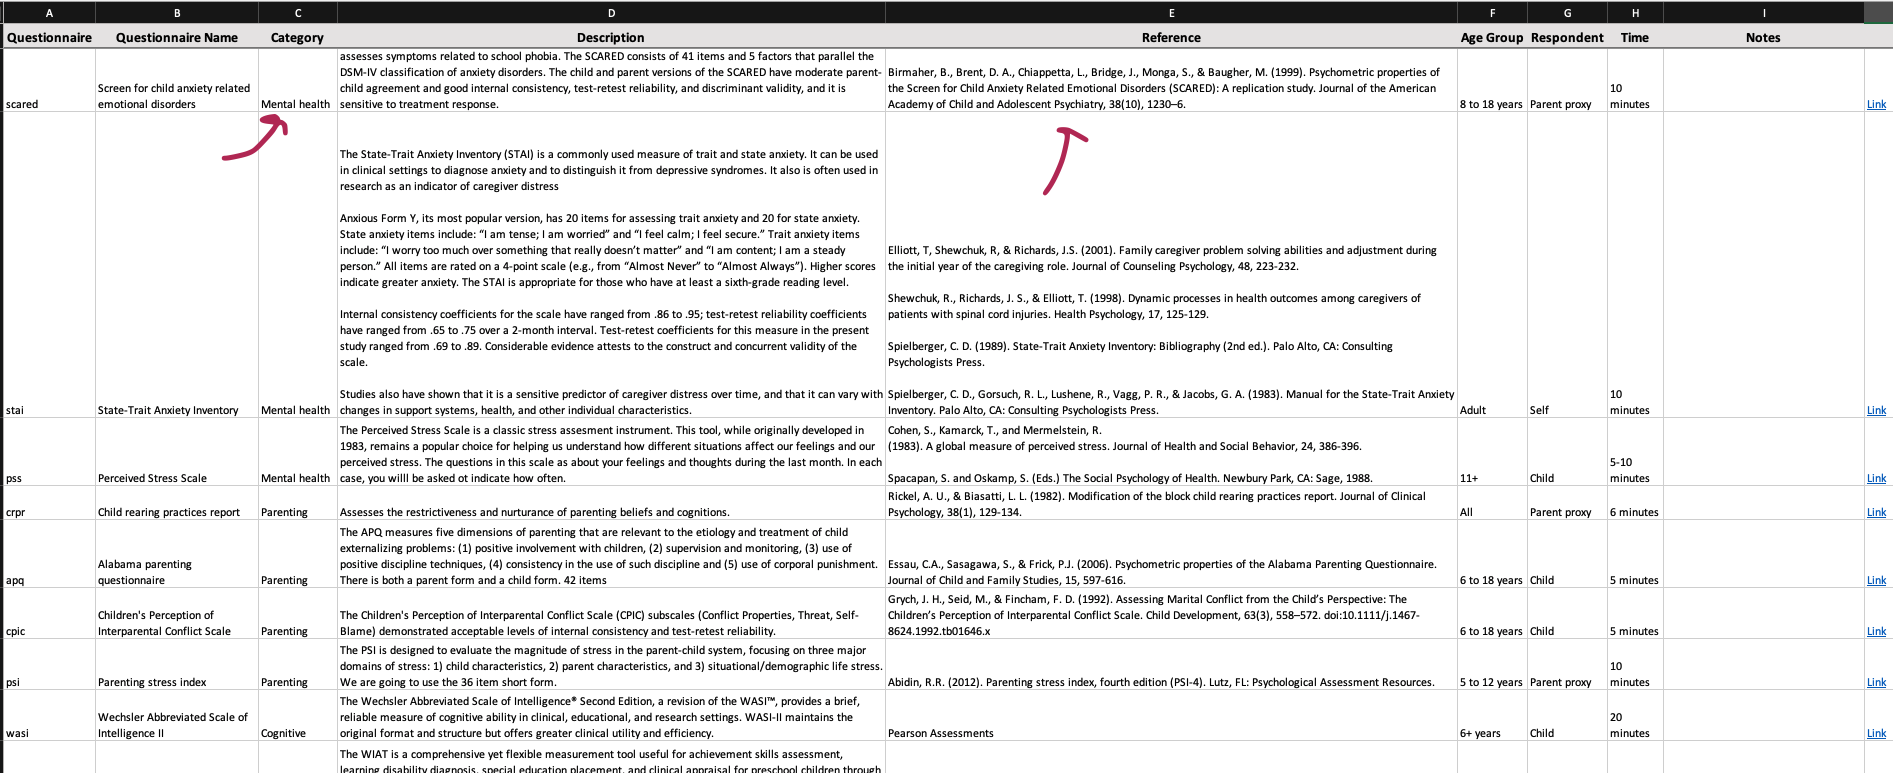
\includegraphics{images/lab_protocols/questionnaire_database/1.png}
\caption{}
\end{figure}

Please create a folder for each questionnaire within the database to allow for the organization of source material. For example, the scq (social cravings questionnaire) was adapted from the fcq (food cravings questionnaire). Therefore, in the scq folder I included the original measure for the fcq, and a paper in which it is desribed and validated. In addition, if you have created this questionnaire as an instrument in REDCap - please upload the zipped file of the instrument to this folder! This will save a great deal of time for future researchers!

\begin{figure}
\centering

\includegraphics{images/lab_protocols/questionnaire_database/2.png}
\caption{}
\end{figure}

\begin{figure}
\centering
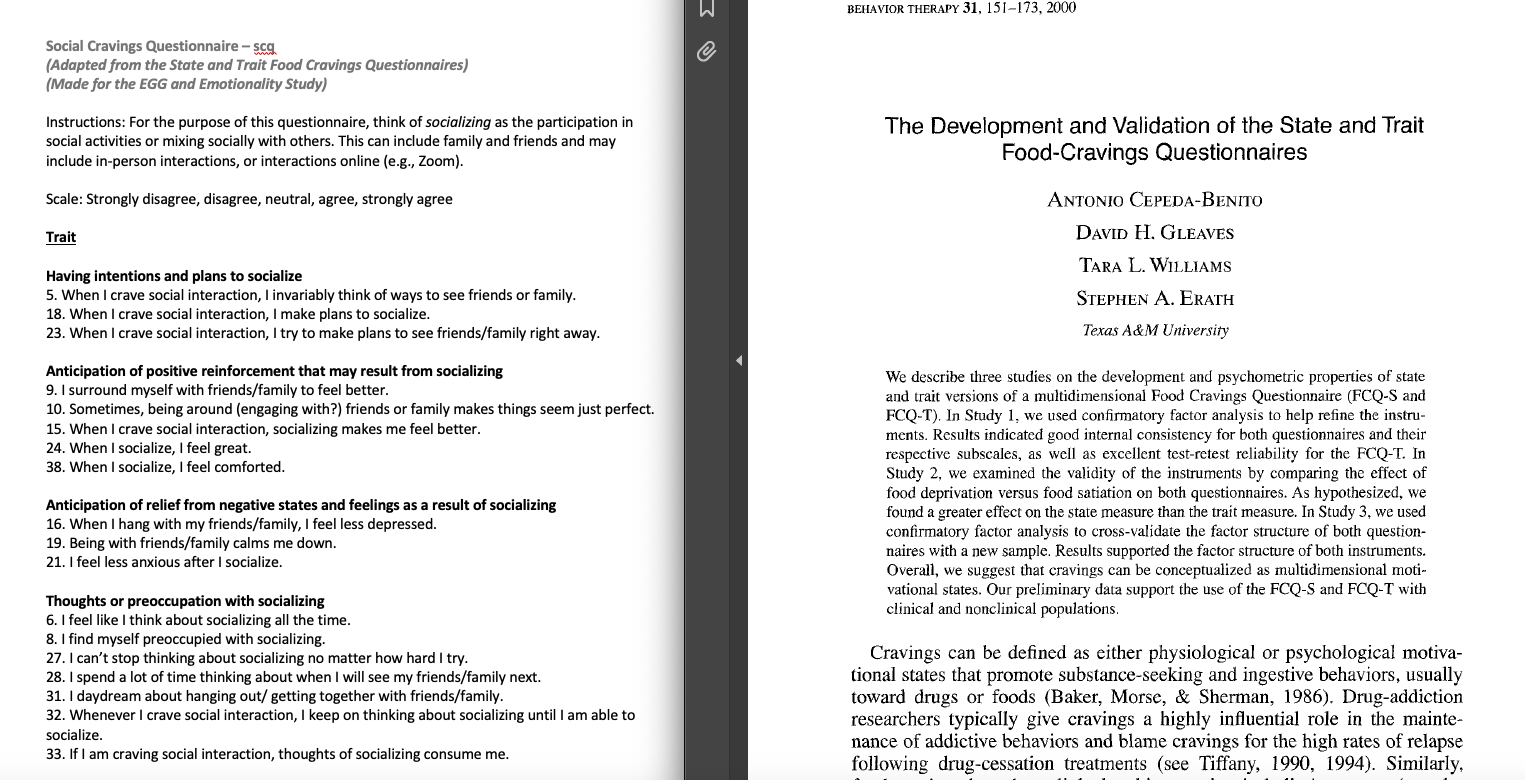
\includegraphics{images/lab_protocols/questionnaire_database/3.png}
\caption{}
\end{figure}

\begin{center}\rule{0.5\linewidth}{0.5pt}\end{center}

\hypertarget{interviews}{%
\section{Interviews}\label{interviews}}

\hypertarget{ksads}{%
\subsection{KSADS}\label{ksads}}

\begin{itemize}
\tightlist
\item
  Align expectations from the start (semi-structured interview)
\item
  Encourage brief responses
\item
  Can write down details later
\item
  Dive in and direct participant
\item
  Read the threshold criteria
\end{itemize}

\begin{center}\rule{0.5\linewidth}{0.5pt}\end{center}

\hypertarget{tests}{%
\section{Tests}\label{tests}}

\begin{center}\rule{0.5\linewidth}{0.5pt}\end{center}

\hypertarget{wasi}{%
\subsection{WASI}\label{wasi}}

\begin{center}\rule{0.5\linewidth}{0.5pt}\end{center}

\hypertarget{wasi-administration}{%
\subsubsection{WASI Administration}\label{wasi-administration}}

Ensure you have all necessary materials (WASI/WIAT administration instruction sheet, WASI score sheet, pencil with NO eraser, WASI administration booklet, WASI score book)

\textbf{Part I: Vocabulary}

\emph{General Instruction}: You will be pointing to each item in the WASI administration booklet and asking the child/adolescent what this item is/if they can describe what this item means to you

\begin{enumerate}
\def\labelenumi{\arabic{enumi}.}
\tightlist
\item
  Start audio recording
\item
  Flip the WASI administration booklet to page 41, item \#4 (what is a shirt?)
\item
  Flip WASI scoring booklet to page 74, beginning with item \#4 (what is a shirt?)

  \begin{itemize}
  \tightlist
  \item
    Use the WASI scoring booklet to determine if child/adolescent's description of each item shall be categorized as score 0, 1, or 2
  \item
    \emph{Note}: Q indicated on the scoring booklet refers to prompt/query the child further- ``Can you tell me more?''
  \item
    Provide queries as often as necessary- marginal responses, generalized responses, functional responses, and gand gestures, but NOT answers that are clearly incorrect
  \end{itemize}
\item
  Note score on the WASI score sheet: Vocabulary
\item
  If the child does not obtain a perfect score on either item 4 or item 5, administer the preceding items in reverse order until two consecutive perfect scores are obtained
\item
  Stop administering when the child/adolescent receives 3 consecutive Zeros \emph{OR} participant hits max score for age group (age 6: item 22; age 7-11: item 25; age 12-14: item 28)
\item
  Keep audio recording for Part II: Matrix Reasoning
\end{enumerate}

\emph{Note: These will be audio recorded and can sometimes move quickly- can be scored later}

\textbf{Part II: Matrix Reasoning}

\emph{General Instruction}: You will be pointing to each matrix reasoning question in the WASI administration booklet and asking the child/adolescent where this item belongs in the missing box

\begin{enumerate}
\def\labelenumi{\arabic{enumi}.}
\tightlist
\item
  Flip the WASI administration booklet to page 57- Practice Questions

  \begin{itemize}
  \tightlist
  \item
    Explain you will do a few practice questions first then walk through 2 practice questions
  \item
    You may acknowledge correct responses/explain why answers may be incorrect
  \end{itemize}
\item
  Flip to correct start page/item to begin (age 6-8: item 1; age 9+: item 4)

  \begin{itemize}
  \tightlist
  \item
    Do NOT give verbal acknowledgement to their answers (e.g.~Correct! That's right!)
  \end{itemize}
\item
  If adolescents age 9+ do not obtain a perfect score on either item 4 or item 5, administer the preceding items in reverse order until two consecutive perfect scores are obtained
\item
  Note score on the WASI score sheet: Matrix Reasoning
\item
  Stop administering when the child/adolescent receives 3 consecutive Zeros \emph{OR} participant hits max score for age group (age 6-8: item 24)
\item
  Stop audio recording
\end{enumerate}

\begin{center}\rule{0.5\linewidth}{0.5pt}\end{center}

\hypertarget{wasi-scoring}{%
\subsubsection{WASI Scoring}\label{wasi-scoring}}

\textbf{Part I}

\begin{enumerate}
\def\labelenumi{\arabic{enumi}.}
\tightlist
\item
  Examiner writes ``scored by: NAME'' at the top of the sheet
\item
  Fill in any missing scores in Vocabulary or Matrix Reasoning tests using audio file if questions are missing (e.g.~scores continue before and after this missing question, NOT because the administrator left questions blank because they have stopped the test)
\item
  Add up the Vocabulary total raw score:

  \begin{itemize}
  \tightlist
  \item
    \emph{Note}: Even if a participant begins at item 4 due to age, the total raw score should still include items 1-3
  \end{itemize}
\item
  Add up Matrix Reasoning total raw score
\item
  Transfer both total raw scores to front sheet under ``Total Raw Score to T-Score Conversion'' chart in column titled ``Raw Score''
\end{enumerate}

\textbf{Part II}

\begin{enumerate}
\def\labelenumi{\arabic{enumi}.}
\tightlist
\item
  Ensure you have the participant's correct age at day of testing in the upper right corner
\item
  Open WASI-II Manual book \textgreater{} page 151 for T-Score Conversions

  \begin{itemize}
  \tightlist
  \item
    Flip to correct chart by age group (age group indicated at top of chart using year:month format)
  \item
    Under the correct chart by age group of the participant, view VC column for Vocabulary and MR column for Matrix Reasoning

    \begin{itemize}
    \tightlist
    \item
      Scroll down VC column for correct Vocabulary total raw score and acquire T-Score equivalent (horizontally)
    \item
      Scroll down MR column for correct Matrix Reasoning total raw score and acquire T-Score equivalent (horizontally)
    \end{itemize}
  \item
    Write T-Score number in the boxes under ``Total Raw Score to T-Score Conversion'' chart in column titled ``T-Scores''

    \begin{itemize}
    \tightlist
    \item
      Add T-Scores totals for box titled ``Full Scale-2''
    \item
      Copy this total number to ``Sum of T-Scores to Composite Score Conversion'' chart in column titled ``Sum of T-Scores''
    \end{itemize}
  \end{itemize}
\item
  Flip WASI-II Manual book \textgreater{} page 188 for FSIQ, Percentile Rank, and Confidence Interval

  \begin{itemize}
  \tightlist
  \item
    \textbf{To obtain FSIQ}: Scroll down Sum of T-Scores column and compare horizontally to FSIQ-2 column
  \item
    \textbf{To obtain Percentile Rank}: Scroll down Sum of T-Scores column and compare horizontally to Percentile Rank column
  \item
    \textbf{To obtain Confidence Interval (always circle/indicate 95\%)}: Scroll down Sum of T-Scores column and compare horizontally to 95\% column in correct age group
  \end{itemize}
\end{enumerate}

\begin{center}\rule{0.5\linewidth}{0.5pt}\end{center}

\hypertarget{wiat}{%
\subsection{WIAT}\label{wiat}}

\begin{center}\rule{0.5\linewidth}{0.5pt}\end{center}

\hypertarget{wiat-administration}{%
\subsubsection{WIAT Administration}\label{wiat-administration}}

Ensure you have all necessary materials (WASI/WIAT administration instruction sheet, WIAT score sheet, 2 pencils with NO erasers, WIAT word reading list, WIAT Math problems sheet)

\textbf{Part I: Word Reading}

\emph{General Instruction}: You will be asking the child/adolescent to read off the WIAT word reading list left to right, top to bottom until they can no longer read the words

\begin{enumerate}
\def\labelenumi{\arabic{enumi}.}
\tightlist
\item
  Start audio recording
\item
  Note in scoring sheet what grade participant is in
\item
  Note the following basic scoring instructions:

  \begin{itemize}
  \tightlist
  \item
    \textbf{(1)} if fluent/correct
  \item
    \textbf{(DK)} if the child does not know
  \item
    \textbf{(\textgreater{}3)} if it took the child longer than 3 seconds to say
  \item
    \textbf{(SC)} if the child said the word wrong but self-corrected
  \end{itemize}
\item
  If multiple attempts are made to read a word, score only the last attempt
\item
  If the child is sounding the word out/verbalizes the word in a choppy manner, ask the child to ``read the word altogether'' immediately after

  \begin{itemize}
  \tightlist
  \item
    If the next attempt is not fluent, score as 0 and say ``try the next one''
  \end{itemize}
\item
  If the child skips a word or row, redirect the child to the appropriate place immediately after and make a note in the scoring sheet
\item
  If the child was unclear when reading a word/you did not hear the child correctly, ask the child to repeat the whole row of words where this particular word was located at the very end after they have finished reading all they can
\item
  Discontinue after the child has reached 4 consecutive Zeros
\end{enumerate}

\textbf{Part II: Numerical Operations}

\begin{enumerate}
\def\labelenumi{\arabic{enumi}.}
\tightlist
\item
  You will be asking the child to fill out the ``math worksheet'' him/herself

  \begin{itemize}
  \tightlist
  \item
    Indicate where to begin based on age (Grades K-1: item 1; grades 2-4: item 14; grades 5-12+: item 18)
  \item
    Explain to the child/adolescent to work on problems from left to right, top to bottom in order and if they do not know a question they may skip it
  \item
    If beginning at item 1, refer to WIAT scoring sheet for specific verbal administration instructions
  \end{itemize}
\item
  If child does not reach 3 consecutive scores of 1, reverse backward until child has reached a correct response
\item
  Be sure to pay attention to the child's responses- if the numbers they write are illegible or mirrored, ask the child to verbally indicate the response they meant

  \begin{itemize}
  \tightlist
  \item
    Note that you obtained a verbal response and note the actual response in your WIAT score sheet
  \end{itemize}
\item
  Discontinue this task when they have reached 4 consecutive Zeros
\item
  Stop audio recording
\end{enumerate}

\begin{center}\rule{0.5\linewidth}{0.5pt}\end{center}

\hypertarget{wiat-scoring}{%
\subsubsection{WIAT Scoring}\label{wiat-scoring}}

\textbf{Part I}

\begin{enumerate}
\def\labelenumi{\arabic{enumi}.}
\tightlist
\item
  Examiner writes ``scored by: NAME'' at the top of the sheet
\item
  Fill in any missing scores in Vocabulary or Matrix Reasoning tests using audio file if questions are missing (e.g.~scores continue before and after this missing question, NOT because the administrator left questions blank because they have stopped the test)
\item
  Add up the Word Reading Total Raw Score:

  \begin{itemize}
  \tightlist
  \item
    Add up Word Reading Total Score Box
  \item
    Add up Total \textgreater{}3" Box
  \item
    Add up Total SC Box
  \end{itemize}
\item
  Word Reading Speed Total Raw Score:

  \begin{itemize}
  \tightlist
  \item
    Listen to the audio file and note time participant began to read words
  \item
    Count 30 seconds forward
  \item
    Note the word the participant completed at 30 seconds; write item number of this word in box
  \end{itemize}
\item
  Add up the Numerical Operations Total Raw Score

  \begin{itemize}
  \tightlist
  \item
    \emph{Note}: Even if a participant begins at item 8 due to age, the total raw score should still include items 1-7
  \end{itemize}
\item
  Transfer both Word Reading Total Raw Score and Numerical Operations Total Raw Score to front page under ``Composite Score Summary'' chart
\end{enumerate}

\textbf{Part II}

\begin{enumerate}
\def\labelenumi{\arabic{enumi}.}
\tightlist
\item
  Ensure you have the participant's correct age at day of testing in the upper right corner
\item
  To obtain the Composite Standard Score:

  \begin{itemize}
  \tightlist
  \item
    Flip WIAT-III Manual book \textgreater{} page 252-387 for Table C.1 based on age of participant (noted at top of chart by year, month, days range)
  \item
    Scroll down Word Reading column and compare horizontally to Standard Score column; write standard score in ``Composite Standard Score'' box
  \item
    Scroll down Numerical Operations column and compare horizontally to Standard Score column; write standard score in ``Composite Standard Score'' box
  \end{itemize}
\item
  To obtain the Confidence Interval (always at 95\%):

  \begin{itemize}
  \tightlist
  \item
    Flip WIAT-III Manual book \textgreater{} page 392 for Table C.3
  \item
    Follow column for correct age \textgreater{} 95\% \textgreater{} Word Reading

    \begin{itemize}
    \tightlist
    \item
      Add and subtract this number to/from the Composite Standard Score: Word Reading to create highest and lowest numbers for the Confidence Interval
    \end{itemize}
  \item
    Follow column for correct age \textgreater{} 95\% \textgreater{} Numerical Operations

    \begin{itemize}
    \tightlist
    \item
      Add and subtract this number to/from the Composite Standard Score: Numerical Operations to create highest and lowest numbers for the Confidence Interval
    \end{itemize}
  \end{itemize}
\item
  To obtain GRADE-LEVEL equivalents of score: (\emph{Note: No longer doing percentile})

  \begin{itemize}
  \tightlist
  \item
    Flip WIAT-III Manual book \textgreater{} page 398 for Table D.2

    \begin{itemize}
    \tightlist
    \item
      Scroll down through Word Reading column and look for raw score, view to left column for grade equivalent
    \end{itemize}
  \item
    Flip WIAT-III Manual book \textgreater{} page 402 for Table D.2

    \begin{itemize}
    \tightlist
    \item
      Scroll down through Numerical Operations column and look for raw score, view to left column for grade equivalent
    \end{itemize}
  \end{itemize}
\end{enumerate}

\begin{center}\rule{0.5\linewidth}{0.5pt}\end{center}

\hypertarget{behavioral-coding}{%
\section{Behavioral Coding}\label{behavioral-coding}}

\begin{center}\rule{0.5\linewidth}{0.5pt}\end{center}

\hypertarget{fims}{%
\subsection{FIMS}\label{fims}}

\begin{itemize}
\tightlist
\item
  Always code positive video first (could be colored by negative video)
\item
  When not obvious use the process of elimination
\item
  Make notes while coding
\item
  Maturity for child for their age
\item
  Attunement = harmonious
\end{itemize}

\begin{center}\rule{0.5\linewidth}{0.5pt}\end{center}

\hypertarget{physiological-measurement}{%
\section{Physiological Measurement}\label{physiological-measurement}}

\begin{center}\rule{0.5\linewidth}{0.5pt}\end{center}

\hypertarget{ecg}{%
\subsection{ECG}\label{ecg}}

Electrocardiogram (ECG) measures a subject's heart rate and waveform pattern. With each heartbeat, an electrical signal travels through the heart. This electrical wave causes the muscle to squeeze and pump blood from the heart. ECG measures this wave through electrodes placed across the torso. By collecting ECG, you can detect changes in heart function due to certain stimuli. Things like stress, excitement, fear, and other emotional responses can be physiologically measured based on changes in the ECG readouts.

\textbf{Biopac Setup}

\begin{itemize}
\tightlist
\item
  In our ECG setup, we have one transmitter with one channel.
\item
  The red and white leads are the signal, the black lead is the ground.
\item
  Because we are using a wireless setup, there needs to be a clear line of sight between the transmitter and the receiver.
\end{itemize}

\textbf{Electrode Placement}

\begin{itemize}
\tightlist
\item
  We will be placing 2 electrodes just below the collarbones and one electrode on the lowest left rib.
\end{itemize}

\textbf{Filtering and Signal Frequency}

\begin{itemize}
\tightlist
\item
  We will sample ECG at a rate of 2kHz, or 2000 samples/second. This gives us a resolution high enough to catch all of the important parts of the heartbeat waveform.
\item
  Noise is not much of an issue with collecting ECG in a 3-electrode setup.
\end{itemize}

\textbf{Subject Position}

\begin{itemize}
\tightlist
\item
  Ensure that the subject is in a comfortable position, so that body movement can be completely avoided or reduced to the minimal. The subject should be asked not to talk, move, read or make phone calls during the procedure.
\item
  Ensure that the position of the subject is the same if there are multiple sessions. Timing of unavoidable body movement or motion artifacts should be noted and the recording periods with motion artifacts must be removed before analysis.
\end{itemize}

\textbf{Gathering ECG Data}

\begin{itemize}
\tightlist
\item
  Lightly abrade the skin at the electrode sites with EL-Prep Gel
\item
  Wipe off excess with a wet wipe or tissue
\item
  After prepping the electrodes with Gel-100, attach electrodes to the skin at the three positions indicated above

  \begin{itemize}
  \tightlist
  \item
    Let these sit as long as possible to adhere and for the gel to soak in
  \end{itemize}
\item
  Ask the participant to put on the module like a belt around their torso

  \begin{itemize}
  \tightlist
  \item
    Make sure the electrode lead inputs are pointed up towards their head
  \end{itemize}
\item
  Connect the white lead to the Right Collarbone electrode, connect the black lead to the Left Collarbone electrode, and connect the red lead to the Left Rib electrode
\item
  Turn on the transmitter and ensure that both the light on the Biopac receiver module and the transmitter are green (the transmitter should be flashing, whereas the receiver should be solid)
\item
  Make sure there is a clear, unobstructed line of sight between the transmitter and receiver antenna
\item
  Open AcqKnowledge by selecting the template file on the desktop

  \begin{itemize}
  \tightlist
  \item
    If the system is not connected to the hardware, make sure the wifi is turned off and restart AcqKnowledge
  \end{itemize}
\item
  Ensure all devices are connected and lead wires attached properly
\item
  Hit the green ``Start'' button and click through all of the dialog boxes that you're prompted with
\end{itemize}

\begin{center}\rule{0.5\linewidth}{0.5pt}\end{center}

\hypertarget{egg}{%
\subsection{EGG}\label{egg}}

\textbf{Biopac Setup}

\begin{itemize}
\tightlist
\item
  In our EGG setup we have one transmitter with two channels (A and B).
\item
  The white leads are the reference, the red are the signal, and the black is the ground.
\item
  Each transmitter needs to have a ground.
\item
  Because we are using a wireless setup, there needs to be a clear line of sight between the transmitter and the receiver.
\end{itemize}

\textbf{Electrode Placement}

\begin{itemize}
\tightlist
\item
  We will place the two white electrodes side-by-side on the xyphoid (which is the lower part of the sternum).
\item
  We will place the two red electrodes in position 1 and 4 in the diagram above.
\item
  We will place the black electrode (the ground) on the second from bottom rib on the left. Try to get it over the bone as much as possible.
\item
  Position 1 should be in line with the reference electrode, and position 4 should be in line with the ground.
\item
  Next, we need to have the transmitter up high on the participants chest so there is line of sight between the transmitter and receiver (antenna).
\end{itemize}

\emph{Alternative}:

\begin{itemize}
\tightlist
\item
  Regular electrocardiogram (ECG) electrodes can be used for EGG recordings.
\item
  The most commonly used configuration for recording 1-channel EGG is to place one electrode at the midpoint on a line connecting the xiphoid and umbilicus, and the other electrode 5 cm away (up and 45 degree) to the patient's left.
\item
  The ground electrode is placed on the left costal margin horizontal to the first active electrode.
\end{itemize}

\textbf{Filtering and signal frequency}

\begin{itemize}
\tightlist
\item
  \emph{Amplification}: the EGG signal is usually in a range of 50-500 μV and adequate amplification needs to be provided by a recording device so that the amplified signal is of an appropriate range for display and analysis
\item
  \emph{Filter setting}: determines the frequency range of the EGG signal to be maximally amplified. The interested range of the EGG signal is in the range of 0.5-9.0 cpm or 0.0083 to 0.15 Hz which is much lower than that of most of extracellular recordings.

  \begin{itemize}
  \tightlist
  \item
    In addition to the basic fundamental frequencies of 0.5-9.0 cpm, it is also important to record certain harmonics (multiples of the fundamental frequency). Accordingly, an appropriate frequency setting is in the range of 0.0083 to 1 Hz.
  \end{itemize}
\end{itemize}

\textbf{Skin Preparation}

\begin{itemize}
\tightlist
\item
  First, the abdominal skin where the electrodes are to be positioned should be thoroughly cleaned to ensure that the impedance between the pair of electrodes is below 10 kΩ.

  \begin{itemize}
  \tightlist
  \item
    To do so, it is advised to abrade the skin until it turns pinkish using some sandy skin-preparation jelly, and then apply a thin layer of electrode jelly for 1 minute for the jelly to penetrate into the skin.
  \end{itemize}
\item
  Before placing the electrode, the excessive jelly must be completely wiped out.
\end{itemize}

\textbf{Subject Position}

\begin{itemize}
\tightlist
\item
  Ensure that the subject is in a comfortable position, most commonly supine, so that body movement can be completely avoided or reduced to the minimal. The subject should be asked not to talk, move, read or make phone calls during the procedure.
\item
  Ensure that the position of the subject is the same if there are multiple sessions. Timing of unavoidable body movement or motion artifacts should be noted and the recording periods with motion artifacts must be removed before analysis.
\end{itemize}

\textbf{Duration of Recording}

\begin{itemize}
\tightlist
\item
  A common mistake in recording the EGG is that the recording is too short. Unlike the ECG in which there are about 60 waves every minute, the EGG is composed of only 3 waves every minute. That is, if the recording is of a short duration of 5 minutes, there are only 15 waves which are obviously insufficient for analysis and interpretation.
\item
  Ideally, at least a 30-minute period is needed to ensure an accurate measure of gastric slow waves in a particular state, such as fasting, fed, baseline or after intervention.
\end{itemize}

\textbf{Meals}

\begin{itemize}
\tightlist
\item
  We will ask participants to eat something about 1 hour before they come into the lab.
\item
  Then we will give them water (as a test meal) immediately before performing the EGG.
\item
  The subjects should all drink the same amount of water.
\end{itemize}

\textbf{Analysis}

\begin{itemize}
\tightlist
\item
  The EGG also contains respiration artifact that is between 12-25 cpm and sometimes the ECG artifacts (< 60 cpm). Occasionally, the slow wave of the small intestine may also be recorded in the EGG (9-12 cpm).
\item
  Although these interferences distort gastric slow waves in the EGG, their frequencies do not overlap with that of the gastric slow waves. Consequently, spectral analysis can be performed to separate the gastric slow waves from interferences.
\item
  Before spectral analysis is performed, any periods with motion artifacts must be identified and deleted because motion artifacts can not be separated from the gastric slow waves even with spectral analysis. So we will need to record their motion during the task.
\end{itemize}

\textbf{Dominant Frequency and Power}

\begin{itemize}
\tightlist
\item
  The dominant frequency and power of the EGG can be derived from the power spectral density assessed by the periodogram method. The normal range of the dominant frequency of the EGG is between 2 to 4 cpm.
\item
  The EGG is called bradygastria if its dominant frequency is lower than 2 cpm, tachygastria if its dominant frequency is higher than 4 cpm but lower than 9 cpm, and arrhythmia if there is no dominant peak power in the spectrum
\end{itemize}

\textbf{Power Ratio or Relative Electrogastrography}

\begin{itemize}
\tightlist
\item
  \emph{Power Change}: The ratio of dominant EGG powers after and before an intervention is a commonly used parameter that is associated with alteration in gastric contractions. It is generally accepted that a ratio of > 1 reflects an increase in gastric contractility due to the intervention, whereas a ratio of < 1 reflects a decrease in gastric contractility.

  \begin{itemize}
  \tightlist
  \item
    If the decibel (dB) unit is used, the ratio should be replaced by the difference between the baseline and after intervention.
  \end{itemize}
\item
  \emph{Percentage of Normal Gastric Slow Waves}: The percentage of normal slow waves is a quantitative assessment of the regularity of the gastric slow wave measured from the EGG. It is defined as the percentage of time during which normal gastric slow waves are observed in the EGG. The percentage of normal slow waves can be computed from the running power spectra of the EGG.

  \begin{itemize}
  \tightlist
  \item
    In this method, 1 spectrum is derived from every 1 minute (or some other short period) of EGG data; the minute is considered normal if its EGG spectrum exhibits a dominant power in the range of 2-4 cpm. In humans, the normal percentage of gastric slow wave is defined as 70\%.
  \end{itemize}
\item
  \emph{Percentage of Gastric Dysrhythmia}: The percentage of gastric dysrhythmia is defined as the percentage of time during which gastric dysrhythmia is observed in the EGG. It is computed in the same way as that for the percentage of normal slow waves.

  \begin{itemize}
  \tightlist
  \item
    It is further classified into the percentage of bradygastria, the percentage of tachygastria and the percentage of arrhythmia.
  \end{itemize}
\end{itemize}

\begin{center}\rule{0.5\linewidth}{0.5pt}\end{center}

\hypertarget{gsr}{%
\subsection{GSR}\label{gsr}}

Electrodermal response (EDR) measurements (including Galvanic Skin Response, GSR) show the activity of the eccrine sweat glands. Typically, one will place electrodes where the concentration of these glands is the highest: namely, the fingertips. The activity of the eccrine sweat glands as a response to physiological excitation (stress, fear, etc.) serves to increase the conductivity of the skin when activated. When one applies a very small electric voltage (0.5 V) between two electrodes, the manifested electrical conductance varies in direct proportion to the electric current flowing between the electrodes. For instance, if a subject is presented a stimulus and the palms start to sweat, this response indicates a highly-stimulated state. The EDR of this subject will then be higher than the subject's baseline. If another subject receives the same stimulus and the palms remain as ``cool as a cucumber,'' the EDA reading will remain unchanged with respect to the baseline. EDR undergoes relatively fast habituation (decrease of amplitude) in the event the same stimulus is repeated over and over to the same subject.

\textbf{Biopac Setup}

\begin{itemize}
\tightlist
\item
  In our GSR setup, we have one transmitter with one channel.
\item
  The red lead is the signal, the black lead is the ground.
\item
  Because we are using a wireless setup, there needs to be a clear line of sight between the transmitter and the receiver.
\end{itemize}

\textbf{Electrode Placement}

\begin{itemize}
\tightlist
\item
  We will be placing the signal electrode on the middle finger of the child's non-dominant hand.

  \begin{itemize}
  \tightlist
  \item
    This has been noted to be the region of the hand with the most concentrated and reactive eccrine sweat glands, and using the non-dominant ensures that the participants will be able to continue with other activities that they may be tasked with while hooked up to the GSR module.
  \end{itemize}
\item
  The ground electrode can be attached anywhere within reach of the transmitter leads. While the above paper grounded to a position on the participant's arm, for the sake of consistency and simplicity, we are attaching the second electrode to the participants' index finger (on the same hand).

  \begin{itemize}
  \tightlist
  \item
    This provides an effective ground, consolidates the leads into one area (preventing potential interference or having the electrodes pulled off by strain on the leads), and also standardizes the placement across all the participants.
  \end{itemize}
\end{itemize}

\textbf{Filtering and Signal Frequency BioPac Recommendation}

\begin{itemize}
\tightlist
\item
  The sample rate can be set quite low for long-term ambulatory measurements or experiments that do not require a high level of temporal precision (i.e., 1-5 samples per second). However, lower sample rates cannot ensure that specific events are accurately represented in what is relayed and graphed, and a degree of timing error might occur.

  \begin{itemize}
  \tightlist
  \item
    To avoid this, BioPac recommends the sampling rate be set to a minimum of 2000 samps/sec (2KHz). Higher sample rates are useful for a number of methodological reasons and for improvements in precision.
  \end{itemize}
\item
  For EDA/GSR measurements, it is typical to filter the data at 35Hz. Some recommendations are that a sample rate of 200Hz - 400Hz are a minimum to ensure enough samples for accurate separation of phasic waveforms from tonic signals and a more accurate representation of signal shape.
\item
  A general approach is to always err on the side of caution and probably seek to sample higher than you really need. As a general rule 1000Hz - 2000Hz sample rates are more than sufficient and easily achievable. The decision for the present study is to collect at a sampling rate of 2000Hz.
\end{itemize}

\textbf{Subject Position}

\begin{itemize}
\tightlist
\item
  Ensure that the subject is in a comfortable position, so that body movement can be completely avoided or reduced to the minimal. The subject should be asked not to talk, move, read or make phone calls during the procedure.
\item
  Ensure that the position of the subject is the same if there are multiple sessions. Timing of unavoidable body movement or motion artifacts should be noted and the recording periods with motion artifacts must be removed before analysis.
\end{itemize}

\textbf{Gathering GSR Data}

\begin{itemize}
\tightlist
\item
  Don't abrade the skin
\item
  After prepping 2 electrodes with a dab of Gel101, attach them to the child's middle and ring fingers

  \begin{itemize}
  \tightlist
  \item
    Let these rest to let the adhesive set and gel soak in for 5 minutes
  \end{itemize}
\item
  Ask the child to put on the PPGED transmitter like a wrist watch. Assist if needed.
\item
  Attach the transmitter leads to the electrodes (red to middle, black to pointer)

  \begin{itemize}
  \tightlist
  \item
    These should be the only two leads connected to the device
  \item
    If there are more leads present, ensure you have the correct transmitter and that the correct lead set is plugged in
  \end{itemize}
\item
  Turn on the transmitter and ensure that both the light on the Biopac receiver module and the transmitter are green (the transmitter should be flashing, whereas the receiver should be solid)
\item
  Make sure there is a clear, unobstructed line of sight between the transmitter and receiver antenna
\item
  Open AcqKnowledge by selecting the template file on the desktop

  \begin{itemize}
  \tightlist
  \item
    If the system is not connected to the hardware, make sure the wifi is turned off and restart AcqKnowledge
  \end{itemize}
\item
  Ensure all devices are connected and lead wires attached properly
\item
  Hit the green ``Start'' button and click through all of the dialog boxes that you're prompted with
\end{itemize}

\begin{center}\rule{0.5\linewidth}{0.5pt}\end{center}

\begin{center}\rule{0.5\linewidth}{0.5pt}\end{center}

\textbf{ECG}

McLaughlin, K. A., Sheridan, M. A., Tibu, F., Fox, N. A., Zeanah, C. H., \& Nelson, C. A. (2015). Causal effects of the early caregiving environment on development of stress response systems in children. \emph{Proceedings of the National Academy of Sciences}, \emph{112}(18), 5637--5642.\\
\url{https://doi.org/10.1073/pnas.1423363112}

\begin{center}\rule{0.5\linewidth}{0.5pt}\end{center}

\textbf{EGG}

Yin, J., \& Chen, J. D. Z. (2013). Electrogastrography: methodology, validation, and applications. \emph{Journal of Neurogastroenterol Motil}, \emph{19}(1), 5-17. \url{http://dx.doi.org/10.5056/jnm.2013.19.1.5}

\begin{center}\rule{0.5\linewidth}{0.5pt}\end{center}

\textbf{GSR}

Braithwaite, J. J., Watson, D. G., Jones, R., \& Rowe, M. (2013). Guide for analysing electrodermal activity (EDA) \& skin conducatance responses (SCRs) for psychological experiments. Technical report: selective attention \& awareness laboratory (SAAL) Behavioural Brain Sciences Centre, University of Birmingham, UK. 1-42. \url{https://www.biopac.com/wp-content/uploads/EDA-SCR-Analysis.pdf}

Martin, I. (1963). Delayed GSR conditioning and the effect of electrode placement on measurements of skin resistance. \emph{Journal of Psychosomatic Research}, \emph{7}(1), 15-22.\\
\url{https://www.sciencedirect.com/science/article/abs/pii/0022399963900473}

\begin{center}\rule{0.5\linewidth}{0.5pt}\end{center}

\bibliography{book.bib,packages.bib}

\end{document}
